\chapter{Marco teórico}
\doublespacing
\section{Antecedentes de estudio}

La asociación Peruana de Ingeniería Hidráulica y Ambiental (APIHA), señaló que en los últimos 60 años ha desaparecido más del 50{\%} del área glaciar del Perú, advierten la existencia de un riesgo enorme de extinción en las siguientes décadas, esto debido al calentamiento global \parencite{gerens}.  Es por ello que especialistas en todo el mundo muestran su preocupación respecto al fenómeno del calentamiento global y sus futuros impactos, entre ellos destaca el retroceso de los glaciares. Para abordar esta problemática, se lleva a cabo numerosos estudios a nivel mundial, enfocándose en el análisis del retroceso glaciar en diversas cordilleras del planeta.

% ################################################################################
Entre las regiones objetivas de atención, las cordilleras del Perú emergen como un área de especial interés. En este contexto, se han llevado a cabo investigaciones específicas en las distintas cordilleras glaciares de nuestro país. Un ejemplo destacado es el estudio realizado por \parencite{navarro20231975}, titulado \textbf{1975--2018: 43 Years of Glacial Retreat in the Incachiriasca Glacier (Nevado Salcantay, Vilcabamba Range, Peru)}. Esta investigación tiene como objetivo el estudio del retroceso del glaciar Incachiriasca, combinando resultados del monitoreo de  2007-2018, con el análisis de 28 imágenes de satélite desde el año 1975-2007. Donde describieron un análisis del retroceso del área glaciar Incachiriasca-II utilizando imágenes del satélite Landsat 2,4,5 y 7 para el análisis de retroceso glaciar, donde se demostró una pérdida del 51.4 {\%} del área total del glaciar, de 0.53 km\textsuperscript{2} (1975) a 0.26 km\textsuperscript{2} (2018) el cual es equivalente a 0.0063 km\textsuperscript{2}/año (1.2 {\%} anual). Según la tendencia del análisis, se observó que la tasa anual del retroceso del glaciar incrementó significativamente, a partir de 2010, aumentando de 1{\%} (2001-2010) a 3 {\%} (2010-2018).

Debido a que los glaciares llegan a ser ecosistemas altamente sensibles al cambio climático, en las últimas décadas los efectos son más evidentes sobre estas reservas de agua sólida, generando una significativa y notoria disminución de la masa glaciar trayendo como efecto la formación de nuevas lagunas, esto es evidenciado en un estudio relizado por \parencite{drenkhan2018current}, titulado \textbf{Current and future glacier and lake assessment in the deglaciating Vilcanota-Urubamba basin, Peruvian Andes}. Este estudio tuvo como objetivo combinar un análisis del desarrollo actual (1988-2016) y futuro (2050-2100) de glaciares y lagos en la cuenca Vilcanota-Urubamba (Cusco, sur de Perú). Los resultados que se obtuvieron indican que el área total de los glaciares disminuyó un 37.35 {\%} de 226.1 km\textsuperscript{2} en 1988 a 141.7 km\textsuperscript{2} en 2016, los lagos adyacentes aumentaron en área un 15.5 {\%} de 23.3 km\textsuperscript{2} (460 lagos) en 1968 a 26.9 km\textsuperscript{2} (544 lagos) en 2016. El estudio supone que las futuras áreas de glaciares podrían disminuir entre un 40.7 {\%} y un 44.9 {\%} en las próximas décadas (2031-2060) y entre un 41.4 {\%} y un 92.7 {\%}, respectivamente, en este siglo (2071­-2100). Por lo tanto, los paisajes andinos se transformarán en áreas en su mayoría libres de glaciares, con algunas cumbres cubiertas de hielo por encima de 6000 msnm. 

En estudios recientes de \parencite{inaigem2023}, ha destacado el valor de los productos satelitales como una fuente crucial de información para el monitoreo y estudio de los glaciares y lagunas. Uno de los proyectos más significativos desarrollados por el INAIGEM fue el \textbf{Inventario Nacional de Glaciares y Lagunas de Origen Glaciar (INGLOG 2)}. Este estudio tuvo como objetivo ofrecer datos clave sobre el estado de los glaciares y las lagunas de origen glaciar en Perú, con el fin de apoyar la toma de decisiones en su gestión. En este inventario, la obtención de información se basó en el uso de imágenes satelitales Sentinel-2, recolectadas durante los meses de menor precipitación y mínima presencia de nubes, optimizando así la calidad y precisión de los datos. Para el procesamiento de estas imágenes, se emplearon herramientas avanzadas de computación en la nube, utilizando plataformas como Google Earth Engine (GEE) y lenguajes de programación como Python y JavaScript, que facilitaron el análisis masivo de datos y la automatización de procesos. En el proceso de segmentación de cuerpos glaciares, se aplicó el Índice Diferencial de Nieve (NDSI), un indicador que mide la diferencia de reflectancia entre el espectro visible verde y el infrarrojo de onda corta. Este índice resultó fundamental para identificar la presencia de nieve y hielo en las imágenes satelitales. Con la ayuda de algoritmos automatizados, se calculó el valor mínimo del NDSI para la colección de imágenes Sentinel-2. Se estableció un umbral mínimo de NDSI >= 0.1, que fue utilizado como indicador de la presencia de cobertura glaciar. Sin embargo, con el objetivo de mejorar la precisión y reducir los márgenes de error en la identificación de glaciares, se implementó una revisión manual adicional. Esta revisión permitió identificar y corregir aquellos índices que, erróneamente, clasificaban sombras, nubes y humedales como parte de la cobertura glaciar. Además, se ajustaron los perímetros glaciales y se rellenaron vacíos internos que no habían sido detectados por el NDSI, mejorando así la confiabilidad de los resultados. Este enfoque híbrido, que combinó algoritmos automatizados con correcciones manuales, permitió obtener una cartografía glaciar más precisa y confiable, sirviendo como base para futuros estudios y estrategias de conservación de los ecosistemas montañosos en Perú.

%Los métodos tradicionales de procesamiento de imágenes basados en información espectral son efectivos y simples, pero requieren mucho procesamiento manual y tiempo, mientras que los métodos recientes basados en inteligencia artificial son más adecuados para terrenos amplios, duros e inaccesibles. 

%Recientemente los algoritmos basados en Machine Learning (ML) están tomando popularidad en aplicaciones de geocicencia

%Los algoritmos de IA pueden manejar automáticamente la dimencionalidad y la complejidad de los datos para ponderar la información de entrada en la clasificación de los límites de los glaciares a través de conjuntos de datos de entrenamiento. El método de segmentación semántica de imágenes, utiliza una red neuronal convolucional (FCN) de aprendizaje profundo esto llega a ser ventajoso, ya que utiliza una estructura de codificación-­decodificación para segmentar el terreno. 
 Recientemente los algoritmos basados en Machine Learning (ML) están tomando popularidad en aplicaciones de geocicencia. Un estudio regional en el uso de Machine Learning para la clasificación de la cobertura glaciar es la tesis de \parencite{garcia2022estimacion}, titulado \textbf{Estimación Del Área Superficial De Un Glaciar Utilizando Técnicas De Procesamiento Digital De Imágenes Satelitales Obtenidas Por El Perusat-1}. El objetivo de este estudio fue calcular la extensión superficial de un glaciar empleando métodos de procesamiento digital de imágenes satelitales captadas por el PeruSat-1 que se enfoca en la estimación del área superficial de glaciares, con un caso de estudio específico en el glaciar Incachiriasca, utilizando procesamiento digital de imágenes satelitales obtenidas por el satélite peruano PeruSAT-1. La metodología aplicada en este trabajo comenzó con un análisis tradicional de monitoreo de glaciares mediante técnicas de procesamiento digital de imágenes, para luego incorporar métodos de Machine Learning, tanto supervisados como no supervisados, que se aplicaron para mejorar la precisión de la clasificación glaciar. Aunque estas técnicas son efectivas, el estudio resaltó que los métodos de Machine Learning son computacionalmente intensivos, lo que dificulta su aplicación a imágenes satelitales de gran tamaño y en escalas más amplias. Para validar los resultados obtenidos, se contrastaron con información proporcionada por el INAIGEM y el Servicio Nacional de Áreas Naturales Protegidas por el Estado (SERNANP). Finalmente, la tesis concluyó con una estimación del área superficial del glaciar Incachiriasca de 16,241.93 m² y una tasa de retroceso glaciar de 4.51 km²/año. Sin embargo, el trabajo también identificó que estos metodos de extracción de cuerpos glaciares enfrentan dificultades para detectar de manera precisa los límites de las superficies glaciares, especialmente en escenarios geográficos complejos. Esto limita su capacidad de ser aplicados de forma automática en cualquier entorno.
 
 Un caso relevante en el uso de técnicas avanzadas de deep learning para la cartografía y monitoreo de masas de agua continentales es el estudio realizado por  \parencite{ghaznavi2024comparative}, titulado \textbf{Comparative performance analysis of simple U-Net, residual attention U-Net, and VGG16-U-Net for inventory inland water bodies}. El objetivo de esta investigación fue desarrollar un método basado en deep learning para inventariar y cartografiar dichas masas utilizando las bandas RGB-NIR (rojo, verde, azul, e infrarrojo cercano) de imágenes satelitales Sentinel-2. En este estudio, se emplearon tres algoritmos de deep learning diferentes, todos basados en la arquitectura U-Net, con el fin de segmentar las masas de agua continentales. Estos algoritmos incluyeron U-Net, Residual Attention U-Net y VGG16-U-Net. Los resultados del estudio indicaron que los algoritmos basados en U-Net son efectivos para inventariar cuerpos de agua de manera rápida, precisa y económica en términos de costo computacional. Esta capacidad de segmentación precisa y eficiente hace que estos métodos sean ideales para aplicaciones a gran escala, permitiendo un análisis eficiente de grandes volúmenes de datos satelitales. Además, los hallazgos de este estudio sientan las bases para la implementación de un mapeo preciso de la cobertura terrestre, utilizando imágenes satelitales. Al proporcionar un algoritmo rápido, objetivo y confiable, este trabajo abre la posibilidad de llevar a cabo inventarios de cobertura terrestre a nivel global con un alto grado de precisión y con menores costos en términos de procesamiento de datos.
 
 Otro estudio realizado por \parencite{rajat2022glacier}, titulado \textbf{Glacier retreat in Himachal from 1994 to 2021 using deep learning}. Cuyo objetivo fue, Aplicar la arquitectura U-Net para la identificación de glaciares, utilizando teledetección proveniente de satélites indios (IRS) y datos satelitales de Landsat, incorporando mejoras en los procesos de segmentación e identificación de glaciares. El cual se hizo en los glaciares de la provincia india de Himachal Pradesh, situada en Himalaya indio occidental, donde se realizó un mapeo glaciar de las últimas tres décadas, es decir, de 1994 a 2021, se evaluó  el impacto del cambio climático utilizando técnicas de segmentación de deep learning en base a imágenes satelitales Landsat 4, 5 y 8, llegando a automatizar el proceso de mapeo de glaciar, el algoritmo utilizado fue U-NET el cual llego a tener una precisión de identificación del 95{\%}, en dicho estudio se observó que el área glaciar de Himachal Pradesh disminuyó a un ritmo de 67,84 km\textsuperscript{2} por año, de 4020,6 km\textsuperscript{2} en 1994 a 2198,5 km\textsuperscript{2} en 2021. Se observa que de 1994 a 2021, el área del glaciar disminuyó aproximadamente en un porcentaje de pérdida de 1,678 por año, con una tendencia decreciente   del 2,31{\%} en 1994 a ­2001 y 1.398{\%} en 2011­ a 2021.
 
 El estudio realizado por \parencite{malone2022evolution}, titulado \textbf{The Evolution of the Two Largest Tropical Ice Masses since
 the 1980s}. El objetivo de esta investigación fue reevaluar el tamaño y las tasas de retroceso de las dos masas de hielo tropicales más grandes: el manto glaciar Quelccaya y el Nevado Coropuna, utilizando datos de la misión Landsat. El análisis se llevó a cabo durante la estación seca, empleando el Índice Diferencial de Nieve Normalizado (NDSI) para segmentar los cuerpos glaciares. Se realizaron correcciones en las imágenes donde el NDSI confundía sombras, nubes y cuerpos de agua con áreas glaciares. Además, se aplicó un umbral de 0.5, que permitió separar de manera más consistente los valores altos, asociados a la nieve, de los valores más bajos atribuidos a otros materiales de la superficie. Para mejorar la precisión, se rellenaron pequeños vacíos en los polígonos (menores de 6000 m²) que habían sido afectados por el umbral, y se eliminaron polígonos pequeños (menores de 10,000 m²), asumiendo que estos representaban coberturas de nieve efímera en lugar de áreas glaciares permanentes. El período de análisis abarcó desde el año 1988 hasta 2020, concluyendo que el manto glaciar de Quelccaya experimentó un notable retroceso desde mediados de la década de 1980. Durante este periodo, el glaciar se redujo en aproximadamente un 26 \%, pasando de 52.60 ± 2.58 km² en 1988 a 39.00 ± 1.92 km² en 2020. La mayor parte de la pérdida de hielo se produjo en elevaciones más bajas, lo que resultó en un aumento de la elevación media del glaciar de 5389 m.s.n.m. a 5449 m.s.n.m.. Esto indica que el manto glaciar de Quelccaya en 2020 es una versión más pequeña, elevada y restringida en comparación con su extensión en 1988. Durante el período de observación (1988-2020), la pérdida total de hielo en el glaciar Quelccaya fue de 13.60 ± 3.22 km², lo que se traduce en una tasa de pérdida media de 0.43 ± 0.10 km² por año. A pesar de esta reducción significativa, el estudio destacó que la tasa de retroceso ha sido relativamente constante a lo largo del tiempo. Finalmente, los hallazgos de este estudio fueron comparados con investigaciones previas sobre glaciares tropicales, concluyendo que ambas masas de hielo tropicales, aunque más pequeñas, se están retirando a un ritmo menor de lo que comúnmente se informa en la literatura científica.

% ###############################################################################

%Entre las regiones objetivas de atención, las cordilleras del Perú emergen como un área de especial interés. En este contexto, se han llevado a cabo investigaciones específicas en las distintas cordilleras glaciares de nuestro país. Un ejemplo destacado es el estudio realizado entre 1975 y 2018 en el Nevado de Salkantay, Cordillera Vilcabamba, Perú, describieron un análisis del retroceso del área glaciar Incachiriasca-II utilizando imágenes del satélite Landsat 2,4,5 y 7 para el análisis de retroceso glaciar, donde se demostró una pérdida del 51.4 {\%} del área total del glaciar, de 0.53 km\textsuperscript{2} (1975) a 0.26 km\textsuperscript{2} (2018) el cual es equivalente a 0.0063 km\textsuperscript{2}/año (1.2 {\%} anual). Según la tendencia del análisis, se observó que la tasa anual del retroceso del glaciar incrementó significativamente, a partir de 2010, aumentando de 1{\%} (2001-2010) a 3 {\%} (2010-2018) \parencite{navarro20231975}. YAAA


%Debido a que los glaciares llegan a ser ecosistemas altamente sensibles al cambio climático, en las últimas décadas los efectos son más evidentes sobre estas reservas de agua sólida, generando una significativa y notoria disminución de la masa glaciar trayendo como efecto la formación de nuevas lagunas, esto es evidenciado en un estudio que tuvo como objetivo combinar un análisis del desarrollo actual (1988-2016) y futuro (2050-2100) de glaciares y lagos en la cuenca Vilcanota-Urubamba (Cusco, sur de Perú). Los resultados que se obtuvieron indican que el área total de los glaciares disminuyó un 37.35 {\%} de 226.1 km\textsuperscript{2} en 1988 a 141.7 km\textsuperscript{2} en 2016, los lagos adyacentes aumentaron en área un 15.5 {\%} de 23.3 km\textsuperscript{2} (460 lagos) en 1968 a 26.9 km\textsuperscript{2} (544 lagos) en 2016. El estudio supone que las futuras áreas de glaciares podrían disminuir entre un 40.7 {\%} y un 44.9 {\%} en las próximas décadas (2031-2060) y entre un 41.4 {\%} y un 92.7 {\%}, respectivamente, en este siglo (2071­-2100). Por lo tanto, los paisajes andinos se transformarán en áreas en su mayoría libres de glaciares, con algunas cumbres cubiertas de hielo por encima de 6000 msnm \parencite{drenkhan2018current}. YAAA


%Según los diferentes escenarios propuestos por del Panel Intergubernamental sobre Cambio Climático (IPCC) para 2050 y 2080, todos los modelos indican que los glaciares continuarán retrocediendo y el permafrost continuará degradándose, lo que resultará en la formación de nuevos lagos glaciares y una mayor susceptibilidad a deslizamientos de tierra \parencite{nullis2018ipcc}. Investigaciones sobre la seguridad hídrica considerando escenarios socioeconómicos y de cambio climático en la cuenca Vilcanota-Urubamba en el periodo (2010-2016), como en corto periodo (2017-2040), mediano (2041-2070) y largo plazo (2071-2099) usando el modelo “Water Evaluation and Planning System (WEAP)” mostraron distintos comportamientos desde un exceso de disponibilidad, pero con una demanda insatisfecha a partir de 2050 en todos sus escenarios \parencite{goyburo2021reconstruccion}. AUNNN


%En estudios recientes \parencite{inaigem2023}, el Instituto Nacional de Investigación en Glaciares y Ecosistemas de Montaña (INAIGEM) ha destacado el valor de los productos satelitales como una fuente crucial de información para el monitoreo y estudio de los glaciares y lagunas. Estos productos permiten la cartografía precisa de la cobertura glaciar, facilitando la observación de detalles importantes como grietas, líneas de nieve, entre otros aspectos relevantes del ecosistema glaciar. YAAAAA

%Uno de los proyectos más significativos desarrollados por el INAIGEM fue el Inventario Nacional de Glaciares y Lagunas de Origen Glaciar (INGLOG 2). En este inventario, la obtención de información se basó en el uso de imágenes satelitales Sentinel-2, recolectadas durante los meses de menor precipitación y mínima presencia de nubes, optimizando así la calidad y precisión de los datos. Para el procesamiento de estas imágenes, se emplearon herramientas avanzadas de computación en la nube, utilizando plataformas como Google Earth Engine (GEE) y lenguajes de programación como Python y JavaScript, que facilitaron el análisis masivo de datos y la automatización de procesos.

%En el proceso de segmentación de cuerpos glaciares, se aplicó el Índice Diferencial de Nieve (NDSI), un indicador que mide la diferencia de reflectancia entre el espectro visible verde y el infrarrojo de onda corta. Este índice resultó fundamental para identificar la presencia de nieve y hielo en las imágenes satelitales. Con la ayuda de algoritmos automatizados, se calculó el valor mínimo del NDSI para la colección de imágenes Sentinel-2. Se estableció un umbral mínimo de NDSI >= 0.1, que fue utilizado como indicador de la presencia de cobertura glaciar.

%Sin embargo, con el objetivo de mejorar la precisión y reducir los márgenes de error en la identificación de glaciares, se implementó una revisión manual adicional. Esta revisión permitió identificar y corregir aquellos índices que, erróneamente, clasificaban sombras, nubes y humedales como parte de la cobertura glaciar. Además, se ajustaron los perímetros glaciales y se rellenaron vacíos internos que no habían sido detectados por el NDSI, mejorando así la confiabilidad de los resultados.
%Este enfoque híbrido, que combinó algoritmos automatizados con correcciones manuales, permitió obtener una cartografía glaciar más precisa y confiable, sirviendo como base para futuros estudios y estrategias de conservación de los ecosistemas montañosos en Perú.


%Los métodos tradicionales de procesamiento de imágenes basados en información espectral son efectivos y simples, pero requieren mucho procesamiento manual y tiempo, mientras que los métodos recientes basados en inteligencia artificial son más adecuados para terrenos amplios, duros e inaccesibles. Recientemente los algoritmos basados en Machine Learning (ML) y Deep Learning (DL) están tomando popularidad en aplicaciones de geocicencia como en el mapeo de deslizamientos de tierra, mapeo de cuerpos de agua, mapeo de lagos glaciares, mapeo de glaciares y delineación de límites de glaciares [A0018], [A0019].  Los algoritmos de IA pueden manejar automáticamente la dimencionalidad y la complejidad de los datos para ponderar la información de entrada en la clasificación de los límites de los glaciares a través de conjuntos de datos de entrenamiento. El método de segmentación semántica de imágenes, utiliza una red neuronal convolucional (FCN) de aprendizaje profundo esto llega a ser ventajoso, ya que utiliza una estructura de codificación-­decodificación para segmentar el terreno. 


%Un estudio regional en el uso de Machine Learning para la clasificación de la cobertura glaciar es la tesis de \parencite{garcia2022estimacion}, que se enfoca en la estimación del área superficial de glaciares, con un caso de estudio específico en el glaciar Incachiriasca, utilizando procesamiento digital de imágenes satelitales obtenidas por el satélite peruano PeruSAT-1. La metodología aplicada en este trabajo comenzó con un análisis tradicional de monitoreo de glaciares mediante técnicas de procesamiento digital de imágenes, para luego incorporar métodos de Machine Learning, tanto supervisados como no supervisados, que se aplicaron para mejorar la precisión de la clasificación glaciar.

%Aunque estas técnicas son efectivas, el estudio resaltó que los métodos de Machine Learning son computacionalmente intensivos, lo que dificulta su aplicación a imágenes satelitales de gran tamaño y en escalas más amplias. Para validar los resultados obtenidos, se contrastaron con información proporcionada por el INAIGEM y el Servicio Nacional de Áreas Naturales Protegidas por el Estado (SERNANP).

%Finalmente, la tesis concluyó con una estimación del área superficial del glaciar Incachiriasca de 16,241.93 m² y una tasa de retroceso glaciar de 4.51 km²/año. Sin embargo, el trabajo también identificó que estos metodos de extracción de cuerpos glaciares enfrentan dificultades para detectar de manera precisa los límites de las superficies glaciares, especialmente en escenarios geográficos complejos. Esto limita su capacidad de ser aplicados de forma automática en cualquier entorno.

%%Estos métodos tradicionales de extracción de cuerpos de agua sufren para detectar de forma precisa los límites de las superficies glaciares sobre todo en escenarios complejos, lo que dificulta su aplicación de forma automática y en cualquier entorno geográfico.

%Un caso relevante en el uso de técnicas avanzadas de deep learning para la cartografía y monitoreo de masas de agua continentales es el estudio realizado por  \parencite{ghaznavi2024comparative}, cuyo objetivo fue desarrollar un método basado en aprendizaje profundo para inventariar y cartografiar dichas masas utilizando las bandas RGB-NIR (rojo, verde, azul, e infrarrojo cercano) de imágenes satelitales Sentinel-2. En este estudio, se emplearon tres algoritmos de aprendizaje profundo diferentes, todos basados en la arquitectura U-Net, con el fin de segmentar las masas de agua continentales. Estos algoritmos incluyeron U-Net, Residual Attention U-Net y VGG16-U-Net.

%Los resultados del estudio indicaron que los algoritmos basados en U-Net son efectivos para inventariar cuerpos de agua de manera rápida, precisa y económica en términos de costo computacional. Esta capacidad de segmentación precisa y eficiente hace que estos métodos sean ideales para aplicaciones a gran escala, permitiendo un análisis eficiente de grandes volúmenes de datos satelitales.

%Además, los hallazgos de este estudio sientan las bases para la implementación de un mapeo preciso de la cobertura terrestre, utilizando imágenes satelitales. Al proporcionar un algoritmo rápido, objetivo y confiable, este trabajo abre la posibilidad de llevar a cabo inventarios de cobertura terrestre a nivel global con un alto grado de precisión y con menores costos en términos de procesamiento de datos.

%Tal es el caso de los estudios realizados por \parencite{rajat2022glacier}. El cual se hizo en los glaciares de la provincia india de Himachal Pradesh, situada en Himalaya indio occidental, donde se realizó un mapeo glaciar de las últimas tres décadas, es decir, de 1994 a 2021, se evaluó  el impacto del cambio climático utilizando técnicas de segmentación de deep learning en base a imágenes satelitales Landsat 4, 5 y 8, llegando a automatizar el proceso de mapeo de glaciar, el algoritmo utilizado fue U-NET el cual llego a tener una precisión de identificación del 95{\%}, en dicho estudio se observó que el área glaciar de Himachal Pradesh disminuyó a un ritmo de 67,84 km\textsuperscript{2} por año, de 4020,6 km\textsuperscript{2} en 1994 a 2198,5 km\textsuperscript{2} en 2021. Se observa que de 1994 a 2021, el área del glaciar disminuyó aproximadamente en un porcentaje de pérdida de 1,678 por año, con una tendencia decreciente   del 2,31{\%} en 1994 a ­2001 y 1.398{\%} en 2011­ a 2021.


%El estudio realizado por \parencite{malone2022evolution} reevalúa el tamaño y las tasas de retroceso de las dos masas de hielo tropicales más grandes: el manto glaciar Quelccaya y el Nevado Coropuna, utilizando datos de la misión Landsat. El análisis se llevó a cabo durante la estación seca, empleando el Índice Diferencial de Nieve Normalizado (NDSI) para segmentar los cuerpos glaciares. Se realizaron correcciones en las imágenes donde el NDSI confundía sombras, nubes y cuerpos de agua con áreas glaciares. Además, se aplicó un umbral de 0.5, que permitió separar de manera más consistente los valores altos, asociados a la nieve, de los valores más bajos atribuidos a otros materiales de la superficie.

%Para mejorar la precisión, se rellenaron pequeños vacíos en los polígonos (menores de 6000 m²) que habían sido afectados por el umbral, y se eliminaron polígonos pequeños (menores de 10,000 m²), asumiendo que estos representaban coberturas de nieve efímera en lugar de áreas glaciares permanentes.

%El período de análisis abarcó desde el año 1988 hasta 2020, concluyendo que el manto glaciar de Quelccaya experimentó un notable retroceso desde mediados de la década de 1980. Durante este periodo, el glaciar se redujo en aproximadamente un 26 \%, pasando de 52.60 ± 2.58 km² en 1988 a 39.00 ± 1.92 km² en 2020. La mayor parte de la pérdida de hielo se produjo en elevaciones más bajas, lo que resultó en un aumento de la elevación media del glaciar de 5389 m.s.n.m. a 5449 m.s.n.m.. Esto indica que el manto glaciar de Quelccaya en 2020 es una versión más pequeña, elevada y restringida en comparación con su extensión en 1988.

%Durante el período de observación (1988-2020), la pérdida total de hielo en el glaciar Quelccaya fue de 13.60 ± 3.22 km², lo que se traduce en una tasa de pérdida media de 0.43 ± 0.10 km² por año. A pesar de esta reducción significativa, el estudio destacó que la tasa de retroceso ha sido relativamente constante a lo largo del tiempo.

%Finalmente, los hallazgos de este estudio fueron comparados con investigaciones previas sobre glaciares tropicales, concluyendo que ambas masas de hielo tropicales, aunque más pequeñas, se están retirando a un ritmo menor de lo que comúnmente se informa en la literatura científica.




\section{Bases teóricas}
	\subsection{Glaciares}
	
	Los glaciares son masas de hielo formadas por nieve compactada y recristalizada en tierra firme, compuestas por cristales de hielo, agua, aire, roca y nieve. Se originan cuando, a lo largo de los años, la acumulación de nieve supera su derretimiento, un proceso común en zonas de alta montaña. A medida que la nieve se comprime, se convierte en hielo, lo que forma el glaciar. Estos cuerpos de hielo se mueven lentamente cuesta abajo de forma continua durante largos periodos.
	
	Los glaciares son dinámicos, ya que sus componentes y funcionamiento varían con el tiempo. Se distinguen tres áreas principales: la Zona de Acumulación, donde el glaciar gana masa; la Zona de Ablación, donde pierde masa a través del derretimiento, generando escorrentías que alimentan los ríos; y la Línea de Equilibrio Altitudinal, que marca el punto donde no hay ganancia ni pérdida de masa. La ubicación de estas zonas cambia en respuesta a las variaciones climáticas \parencite{menzies1995modern}, \parencite{ceballos2012glaciares}, \parencite{inaigem2023}.
	
	\begin{figure}[h!]
		\centering
		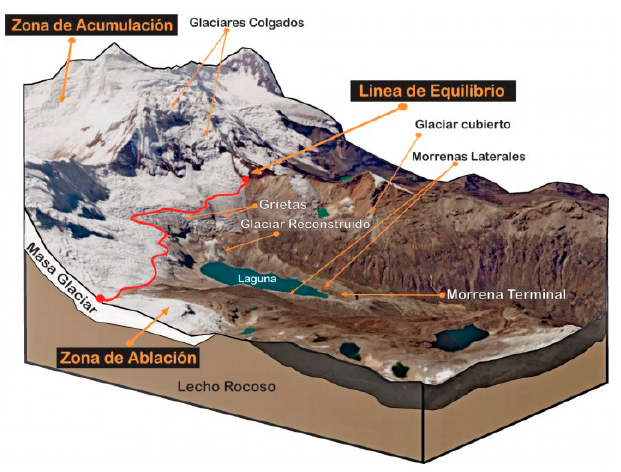
\includegraphics[width=0.7\linewidth]{graficos/glaciar_componentes}
		\caption [Componentes circundantes de un glaciar.]{Componentes circundantes de un glaciar. 
			
			Fuente: \parencite{inaigem2023}}
		\label{fig:glaciar_componentes}
	\end{figure}
	
	\subsubsection{Glaciares Tropicales}
	
	Los glaciares tropicales son aquellos ubicados en latitudes cercanas al ecuador, entre los trópicos de Cáncer y Capricornio. Aproximadamente el 99 \% de estos glaciares a nivel mundial se concentra en la cordillera de los Andes, abarcando territorios de países como Venezuela, Colombia, Ecuador, Perú, Bolivia, Chile y Argentina.
	
	Perú alberga el 68 \% de los glaciares tropicales del mundo \parencite{veettil2017remote}, distribuidos en 20 cordilleras a lo largo de las regiones norte, centro y sur del país. Estos glaciares son de gran relevancia debido a su sensibilidad al cambio climático, lo que los convierte en excelentes indicadores de las variaciones climáticas \parencite{francou1999symptoms}.
	\begin{figure}[h!]
		\centering
		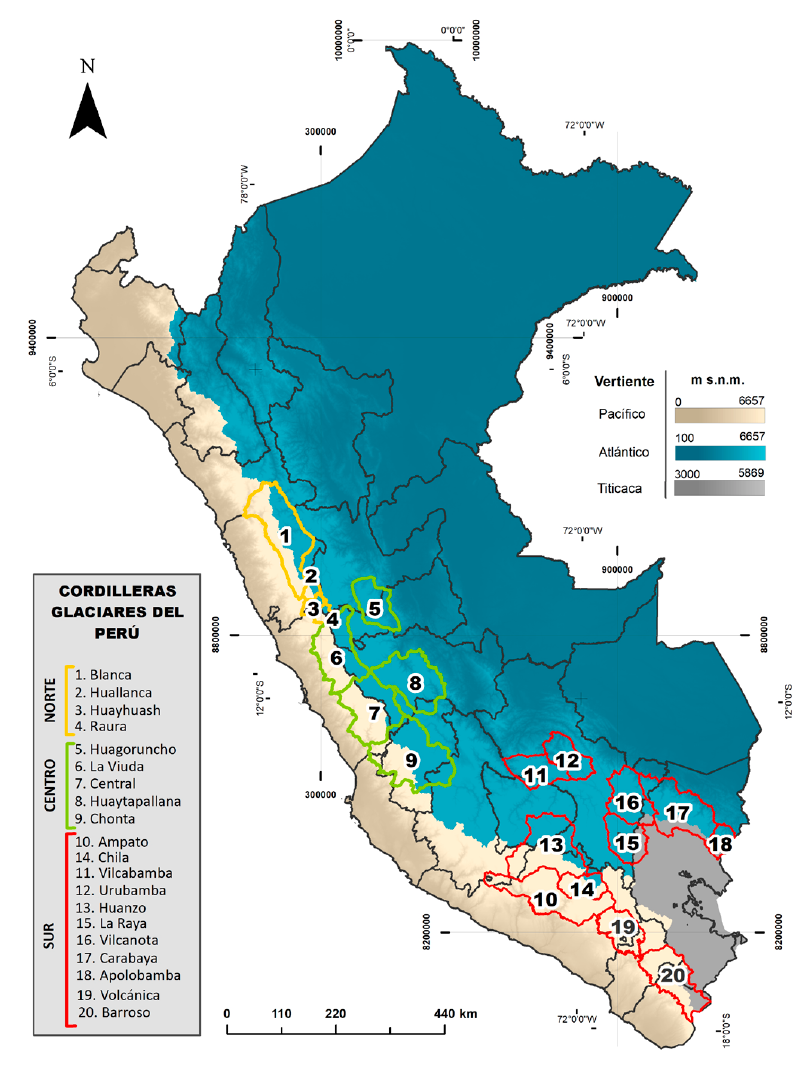
\includegraphics[width=0.7\linewidth]{graficos/cordilleras_peru}
		\caption [Localización de las cordilleras glaciares en el Perú.]{Localización de las cordilleras glaciares en el Perú. 
			
			Fuente: \parencite{inaigem2023}}
		\label{fig:cordilleras_peru}
	\end{figure}
	\subsubsection{Clasificación de los glaciares tropicales}
	Cada glaciar poseee caracteristicas particualres,segun INAIGEM clasifico cada glaciar por tipo d superficie: Glaciar libre de detritos, glaciar cubierto por detritos y glaciar rocoso. 
	
	\begin{enumerate}
		\item[a)] \textbf{Glaciar libre de detritos:} Son glaciares que no presentan un alto grado de impurezas o material particulado en su superficie; sin embargo, en algunos casos pueden contener un pequeño porcentaje de material detrítico, cenizas o impurezas \parencite{lliboutry1956}. Este material se acumula en la superficie del glaciar debido al transporte de partículas por los vientos, las cuales provienen del desprendimiento de laderas cercanas.
		
		\item[b)] \textbf{Glaciar cubierto por detritos:} Su característica principal es que están parcial o totalmente cubiertos por una capa de detritos supraglaciares. A diferencia de los glaciares libres de detritos, el material detrítico proviene principalmente de la fragmentación de rocas causada por procesos de meteorización \parencite{anderson2016modeling}.
		
		\item[c)] \textbf{Glaciar rocoso:} Está formada principalmente por detritos, rocas y hielo que se desplazan cuesta abajo debido a la gravedad. Su característica más notable es la aparición de surcos y lóbulos en la superficie. En los glaciares rocosos, el hielo no suele aflorar en la superficie, ya que está presente en los espacios internos entre los escombros o confinado en un núcleo de hielo en el interior \parencite{potter1972ice}.
	\end{enumerate}
	
	\subsection{Retroceso glaciar}
	Se define como retroceso glaciar al ascenso de la línea inferior de los glaciares de alta montaña cada vez hacia áreas de altitud más alta o latitudes más frías generando una disminución en su extensión, espesor y volumen de la masa glaciar a lo largo del tiempo, El retroceso glaciar ocurre por el desequilibrio entre la acumulación de hilo y nieve en la parte superior del glaciar (zona de acumulación) y la pérdida de hielo en la parte inferior (zona de ablación) \parencite{delretroceso}.
	
	\subsection{Principales causas del retroceso glaciar}
	\subsubsection{Cambio climático}
	
	El Panel Intergubernamental sobre Cambio Climático (IPCC, por sus siglas en inglés) define el cambio climático como una modificación en el estado del clima que se manifiesta en un cambio del valor promedio y/o en la variabilidad de sus propiedades, y que perdura durante un período prolongado \parencite{ipcc2019}.
	
	Asimismo, el IPCC advierte sobre un rápido y significativo cambio en los glaciares de todas las regiones, incluidos los Andes tropicales. En general, los estudios indican una tendencia de reducción en la cobertura glaciar en las últimas décadas \parencite{inaigem2023}.
	
	El grado de retroceso varía según las características de cada glaciar, siendo los más pequeños y a menor altitud los más vulnerables. Sin embargo, comprender la relación entre el retroceso glaciar y el cambio climático es complejo, ya que la dinámica glaciar está influenciada tanto por factores locales, como la pendiente y orientación del glaciar, como por características climáticas regionales. Además, se prevé que la cantidad de lagunas glaciares continuará aumentando. También se estima que, para finales del 2100, el caudal de las cuencas podría reducirse en un 10 \% o más durante las temporadas secas en zonas montañosas \parencite{ipcc2019}.
	
	\subsubsection{Contaminación por particulas absorbentes de luz}
	Además del cambio climático, los glaciares están siendo influenciados por las llamadas "partículas absorbentes de luz", como el carbono negro, carbono orgánico y polvo mineral. Estas partículas, transportadas por el viento desde sus fuentes, terminan depositándose sobre la superficie glaciar. Al estar en la superficie, reducen el albedo de la nieve, lo que provoca una mayor absorción de energía solar, incrementando el calor y acelerando el derretimiento de los glaciares \parencite{bond2013}, \parencite{gilardoni2022}.
	
	El principal componente de las partículas absorbentes de luz es el carbono negro (figura 12), que tiene un impacto significativo en los glaciares, ya que incluso en pequeñas cantidades puede alterar el balance energético en la superficie de la nieve \parencite{inaigem2023}. Este tipo de partículas se generan por la combustión incompleta de combustibles fósiles y biomasa, como ocurre con las emisiones de vehículos, industrias, incendios forestales y la quema de residuos \parencite{bond2013}.
	
	En la cordillera Blanca, se ha observado que las altas concentraciones de partículas absorbentes de luz están relacionadas con la cercanía a áreas urbanas. Además, estudios en las cordilleras Blanca, Huaytapallana y Vilcanota han demostrado que la mayor deposición de estas partículas sobre los glaciares ocurre entre el invierno y la primavera, coincidiendo con la temporada seca \parencite{torres2018}, \parencite{inaigem2023}.
	
	\begin{figure}[h!]
		\centering
		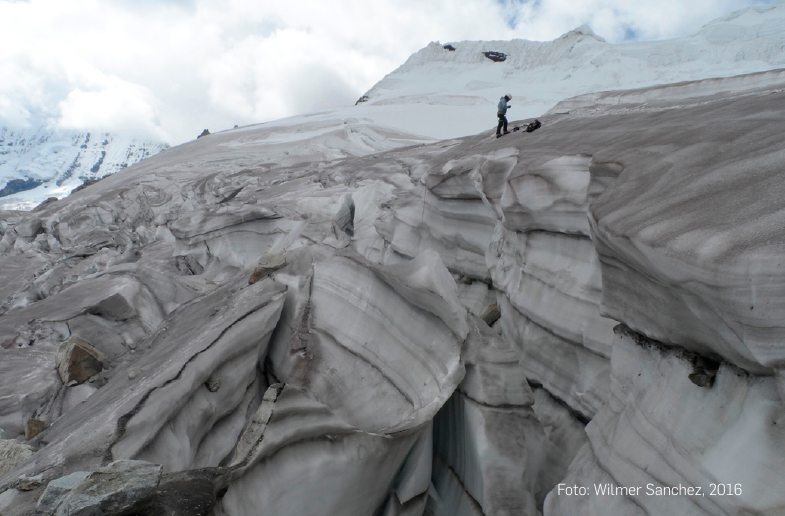
\includegraphics[width=0.7\linewidth]{graficos/carbonoNegro}
		\caption[Carbono negro en la superficie del glaciar Yanapaccha, cordillera Blanca.]{Carbono negro en la superficie del glaciar Yanapaccha, cordillera Blanca. 
			
			Fuente: \parencite{inaigem2023}}
		\label{fig:carbonoNegro}
	\end{figure}
	
	%El casquete de hielo Quelccaya se asienta sobre una meseta de gran altitud en la cordillera de los Andes de Perú, Sin embrago las temperaturas comprativamenete frías que se encuentran a grandes altitudes no son los suficientes para protegerlo del cambio climatico.
	%En la figura se muestra el retroces del borde de hiel del glaciar Quelccaya entre el 3 de deptiembre de 1988 y el 22 de octubre de 2023. Christopher Shuman, glaciólogo de la UNiversidad de Maryland, condado de Balatimore, y que trabaja en el Centro de Vuelo de la NASA, estima que el área del hielo en 1988 se extedia por unos 58 kilometros cuadrados (22 millas cuadradas); en 2023, abarca aproximadamente 40 kilometros cuadraos (15 millas cuadradas)
	
	%Algunos de los lagos ya han ido apareciendo y desapareciendo durante el periodo de tiempo que abarca estas imágenes, incluso uno que en noviembre 2022 produjo una inundación ppor el desbordamiento violento de un lago glaciar. Shuman detecto el suceso en imagenes de Landsat que mostraban el vaciamiento de un lago en el lado este del casquete de hielo y un largo camino donde el agua de la inundación habia arrazado la vegetación. La cicatris de la inundación es visible en la imagen del 2023
	
	%Antes de que los sátelites Landsat revelaran los cambios decenales, los cientificos ya ssbian que el casquete de hielo ya se estaba reduciendo. Desde 1974, Lonnie Thompson y sus clogas de la universidad de Ohio han estado organizando expediciones para estudiar el Quelccaya.
	
	%Tanto las imágenes terrestres como las satelitales permiten documentar las tasas de retroceso de los glaciares, que ahora promedian unos 14 metros por año, dijo Thompson. El equipo de thompson ha compartido las imagenes de Landsat que documentan el retroceso del casquete del Glaciar Quelccaya, a medida que se van perdiendo los glaciares tropicales del planeta, también se estan perdiendo los registros de temperatura y clima conservados por mucho tiempo en sus hielos. El equipo ha perforado núcleos de hielo de muchos glaciares tropicales, incluidos el Quelccaya. Al analizar las capas de estos núcleos, los científicos pueden obtener un registro casi anual de las temperaturas del aire y la compoosición atmosferica que se remonta a 1.800 años en el pasado.
	
	%“Los glaciares tropicales podrían representar nuestra única oportunidad de captar los cambios de la temperatura media global a lo largo del tiempo, así como la forma en que el clima y el medioambiente han cambiado en un área que representa el 50 por ciento de la superficie de nuestro planeta y donde vive más del 50 por ciento de nuestros 8.000 millones de habitantes”, dijo Thompson.
	
	%En Quelccaya ese record podria desparecer a finales del siglo 21, que es el plazo previsto para la desaparición del casquete de hielo. "La única prueba de su existencia serán las imágenes terrestres y satelitales se lo que alguna vez fue un mágnifico casquete de hielo ubicado directamente sobre la cuenca del Amazonas. 
	
	\subsection{Teledetección}
	Los fenómenos que ocurren sobre la superficie de la tierra, tienen un gran interés por parte de la comunidad científica, esto ha llevado a realizarse muchísimos estudios en las últimas décadas, se tiene un interés sobre lo que sucede en la atmosfera, océanos y la superficie de la tierra. Para poder evaluar, analizar y predecir estos fenómenos se tienen que monitorizar ciertos parámetro que llegan a relacionarse de manera directa o indirecta con procesos geofísicos y biofísicos. Es en este punto donde la técnica de teledetección toma un papel importante, puesto que nos permite medir dichos parámetros de forma remota sin tener la necesidad de entrar en contacto directo con la superficie terrestre. 
	Según la Agencia Espacial Europea \parencite{sobrino2001teledeteccion} define la teledetección como la técnica de recopilar, evaluar y analizar datos de un objeto para obtener información de este sin necesidad de estar en contacto directo con el objeto de estudio. A su vez se tienen que distinguir tres elementos esenciales para la teledetección, que llegan a ser:
	
	\begin{enumerate}
		\item Una plataforma que transporta los instrumentos.
		\item Fuente de energía.
		\item Medio de propagación.
		\item Un objeto de observación.
		\item Un instrumento o sensor que observe el objeto.
		\item Sistema receptor.
		\item Usuario.
	\end{enumerate}
	
	La técnica de teledetección utiliza las propiedades que tienen los objetos para radiar energía, de esta manera obtener información del cuerpo observado.
	
	\subsection{Radiación electromagnética}
	La radiación electromagnética se puede caracterizar atreves de su frecuencia y por su longitud de onda como: ondas de radio, microondas, infrarrojo, luz visible, ultravioleta, rayos X, rayos gamma, etc. Las longitudes de onda son continuas, pero pueden agruparse en bandas sin límites definidos, a esto se le conoce como espectro electromagnético. Tal como podemos observar en la Figura \ref{fig:espectro1}, comprendido desde ondas pequeñas como los rayos gamma hasta ondas de mayor longitud como las ondas de radio \parencite{halliday2015physics}.
 
	
	\begin{figure}[h!]
		\centering
		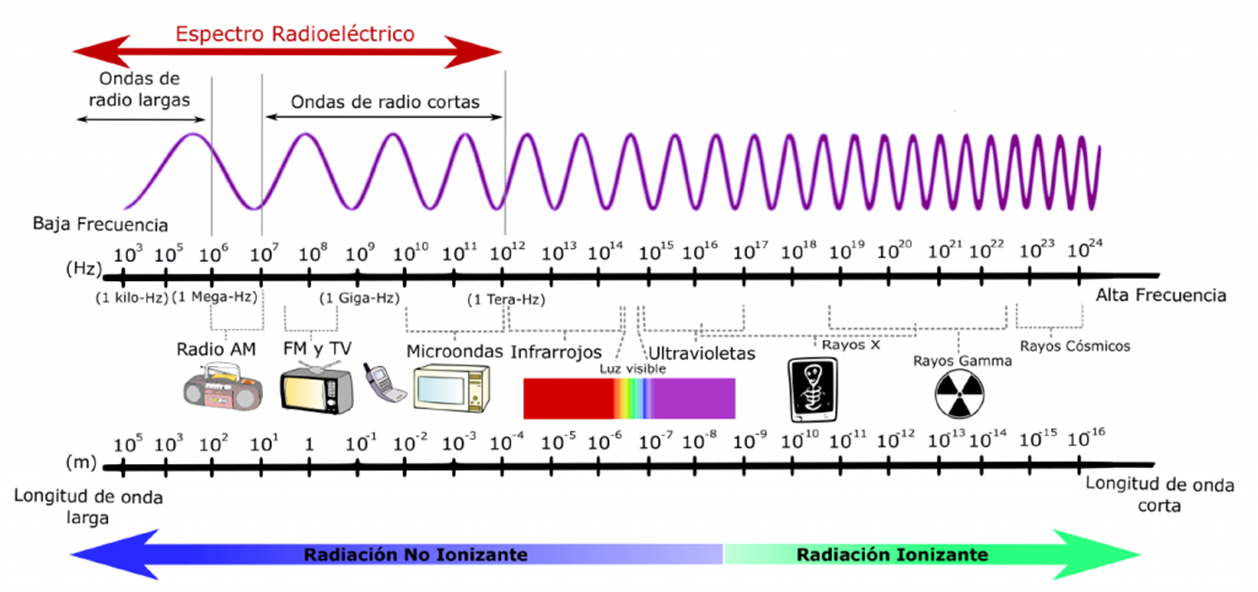
\includegraphics[width=0.9\linewidth]{graficos/espectro1}
		\caption[Espectro electromagnético basada en el rango de longitud de onda y frecuencia.]{Espectro electromagnético basada en el rango de longitud de onda y frecuencia. 
			
			Fuente: \parencite{rojas2013radiacion}}
		\label{fig:espectro1}
	\end{figure}
	
	Normalmente en teledetección utiliza una serie de bandas que llegan a ser más útiles que otras, como:
	
	
	\textbf{Espectro visible (VIS): } Componen de longitudes de onda que varían en el rango de \( (\lambda \text{ de } 0.4 \text{ a } 0.7 \mu m) \): compone tres bandas fundamentales, rojo \( (\lambda \text{ de } 0.6 \text{ a } 0.7 \mu m) \), verde \( (\lambda \text{ de } 0.5 \text{ a } 0.6 \mu m) \) y azul \( (\lambda \text{ de } 0.4 \text{ a } 0.5 \mu m) \), además esta porción del espectro es el rango completo de la energía electromagnética, al cual es sensible al ojo humano \parencite{halliday2015physics}.
	
	\textbf{Infrarrojo cercano (NIR): } Componen de longitudes de onda que varían en el rango de \( (\lambda \text{ de } 0.7 \text{ a } 1.3 \mu m) \) esta porción del espectro permite discriminar masas vegetales asi como las concentraciones de humedad \parencite{halliday2015physics}.
	
	\textbf{Infrarrojo de onda corta 1 (SWIR-1): } Componen de longitudes de onda que varían en el rango de \( (\lambda \text{ de } 1.57 \text{ a } 1.65 \mu m) \), se emplea para discriminar el contenido de humedad en la vegetación o en los suelos \parencite{halliday2015physics}. 
	
	\textbf{Infarrojo de onda corta 2 (SWIR-2): } Componen de longitudes de onda que varían en el rango de \( (\lambda \text{ de } 2.08 \text{ a } 2.35 \mu m) \), se emplea para discriminar propiedades del agua, minerales, etc \parencite{halliday2015physics}.
	
	\textbf{Infrarrojo termico (TIRS): } Componen de longitudes de onda que varían en el rango de \( (\lambda \text{ de } 8 \text{ a } 14 \mu m) \), decisivo para localización de lugares con alta temperatura se emplea para localizar el calor proveniente de gran parte de las cubiertas terrestres \parencite{halliday2015physics}.
	
	\subsection{Interacción de la radiación con la atmosfera}
	Antes de que la radiación electromagnética llegue a la superficie terrestre, ocurren tres interacciones en la atmosfera, absorción, transmisión y dispersión.
	\subsubsection{Absorción atmosferica}
	La energía electromagnética que viaja a través del espacio en dirección a la atmosfera es parcialmente absorbida por varias moléculas, destacando en la absorción: Ozono (O3), Vapor de agua (H2O), oxígeno molecular O2, dióxido de carbono (CO2) y aerosoles atmosféricos \parencite{geotig}, cada uno de ellos absorbe energía en distintos rangos del espectro, como se puede observar en la Figura \ref{fig:TransAtmos}. Además se observa que existe una gran cantidad de longitudes de onda que no son útiles, puesto que no pueden penetrar la atmosfera. 
	
	
	\begin{figure}[h!]
		\centering
		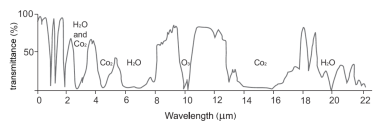
\includegraphics[width=0.7\linewidth]{graficos/TransAtmos}
		\caption[Transmisión Atmosférica.]{Transmisión Atmosférica. 
			
			Fuente: \cite{camps2011remote}}
		\label{fig:TransAtmos}
	\end{figure}
	
	
	En la Figura \ref{fig:VentanasAtmosfericas} el color gris indica bandas de absorción y las áreas azules indican ventanas atmosféricas, es lo que los sensores de los satélites son capaces de ver en la superficie terrestre.
	Las ventanas de 0.4 a 2 µm la radiación en este rango es (Visible, NIR, SWIR) es principalmente energía reflejada. Los sensores que operan en este rango a menudo son llamados ópticos.(Tempfli et al., 2009)
	
	\begin{figure}[h!]
		\centering
		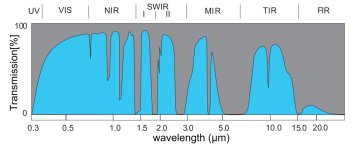
\includegraphics[width=0.7\linewidth]{graficos/VentanasAtmosfericas}
		\caption[Ventanas Atmosféricas en Imágenes Ópticas Multiespectrales.]{Ventanas Atmosféricas en Imágenes Ópticas Multiespectrales. 
			
			Fuente: \parencite{camps2011remote}}
		\label{fig:VentanasAtmosfericas}
	\end{figure}
	
	\subsubsection{Dispersión}
	La dispersión sucede cuando la radiación llega a interactuar con partículas en suspensión, tales como aerosoles y moléculas de aire. Estas partículas llegan a desviar la trayectoria de la radiación en diferentes direcciones, provocando que la luz sea dispersado en todo el espectro electromagnético \parencite{geotig}.
	
	\begin{comment}
	\subsection{Curvas de reflactancia espectral}
	
	Cada material de la superficie terrestre tiene una curva característica de reflectancia, esta curva muestra la porción de energía incidente que es reflejada en función de su longitud de onda, tal como se puede observar en la Figura \ref{fig:CurvasReflejtancia}.
	
	\begin{figure}[h!]
		\centering
		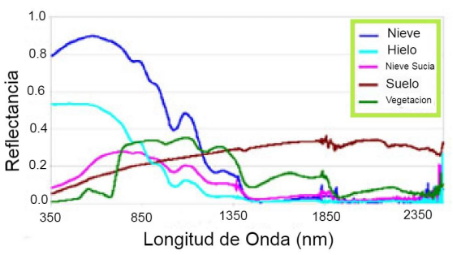
\includegraphics[width=0.7\linewidth]{graficos/CurvasReflejtancia}
		\caption[Curvas de reflectancia espectral de diferentes coberturas.]{Curvas de reflectancia espectral de diferentes coberturas. 
			
			Fuente: \parencite{camps2011remote}}
		\label{fig:CurvasReflejtancia}
	\end{figure}
	\end{comment}

	\subsection{Resolución de imágenes}
	
	\subsubsection{Resolución espacial}
	Es el objeto más pequeño que se puede llegar a identificar en una imagen. Generalmente, se describe como el campo de visión
	instantáneo se define como el Angulo de visión máxima en el que un sensor puede
	detectar eficazmente la energía electromagnética \parencite{camps2011remote}.
	
	\subsubsection{Resolución espectral}
	Es el número de bandas que tiene el sensor, la longitud onda de las bandas, las posiciones en que se ubican las bandas en el espectro electromagnético. Una alta resolución espectral proporciona una firma espectral más precisa \parencite{camps2011remote}.
	
	\subsubsection{Resolución radiométrica}
	Es la capacidad para detectar variaciones en la radiancia espectral que recibe. Está determinado por el número de niveles discretos en los que se puede dividir la radiación de la señal \parencite{camps2011remote}. Cuanto sea mayor la resolución radiométrica podrá interpretarse mejor la imagen \parencite{chuvieco1996fundamentos}.
	\subsubsection{Resolución temporal}
	Es la frecuencia de cobertura que proporciona el sensor. Se refiere a la frecuencia con la que el sensor vuelve a visitar un área y toma imágenes periódicamente durante su vida útil \parencite{meneses2012introduccao}.
	
	\begin{comment}
		\subsection{Programa Satélite Landsat 8}
		Según \parencite{ldcm-l8}, antes de 1972, la idea de utilizar satélites para la vigilancia terrestre, la cartografía o la exploración era una visión futurista. Sin embargo, esto dio origen al Programa Landsat, una serie de misiones de observación de la Tierra gestionadas por la NASA y el Servicio Geológico de Estados Unidos (USGS). Desde su inicio en 1972, Landsat ha revolucionado el estudio de nuestro planeta, proporcionando la serie más extensa de datos satelitales sobre los cambios en la superficie terrestre.
		
		Actualmente, el programa está en su octava misión, conocida como "Landsat Data Continuity Mission" (LDCM) o Landsat 8. Este satélite cuenta con dos segmentos principales: el observatorio, que incluye los sensores OLI (Operational Land Imager) y TIRS (Thermal Infrared Sensor) para capturar imágenes de la Tierra, y el sistema terrestre, que gestiona la planificación, administración y distribución de datos. El satélite sigue la misma trayectoria que sus predecesores, permitiendo la continuidad de los registros de datos a lo largo del tiempo.
		
		Landsat 8 produce imágenes con nueve bandas espectrales, la mayoría con una resolución de 30 metros, y una banda pancromática con una resolución de 15 metros. Las bandas térmicas permiten medir con precisión las temperaturas de la superficie, mientras que las nuevas bandas son útiles para estudios costeros y detección de nubes cirrus. Las imágenes cubren una extensión de aproximadamente 170 km de norte a sur y 183 km de este a oeste.
		
		\subsubsection{Sensor OLI}
		
		El sensor Operational Land Imager (OLI) representa un avance en la tecnología de sensores Landsat, siguiendo el modelo del sensor Advanced Land Imager del satélite experimental EO-1 de la NASA. Mientras que los primeros satélites Landsat usaban sensores tipo "whiskbroom", que utilizaban espejos para barrer el campo espectral, el OLI emplea una tecnología "pushbroom". Este diseño consta de una larga serie de más de 7,000 detectores por banda espectral alineados en el plano focal, lo que permite captar mejor la luz sin necesidad de partes móviles. Esto hace que el OLI sea más sensible y eficiente, proporcionando datos más detallados de la superficie terrestre.
		
		El OLI produce imágenes con una resolución espacial de 15 metros para las bandas pancromáticas y 30 metros para las bandas visibles, infrarrojas cercanas e infrarrojas de onda corta. Las imágenes permiten una observación detallada de zonas amplias de la Tierra, como áreas urbanas, agrícolas y forestales. El OLI fue diseñado para tener una vida útil de cinco años, la matriz del plano focal (FPA) se compone de un sensor con 14 chips ensamblados (SCA). Ademas cada SCA contiene 494 detectores de 12 pixeles de video de referencia que no responden a la luz. Todas las bandas con las que cuenta el sensor OLI adquieren 12 bits de resolución radiométrica \parencite{ldcm-l8}. 
		
		\begin{figure}[h!]
			\centering
			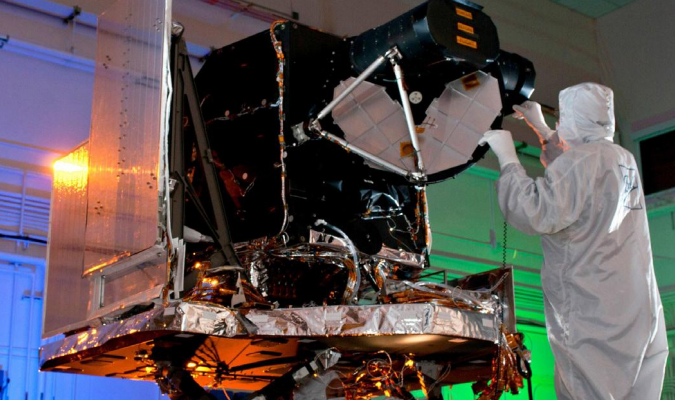
\includegraphics[width=0.7\linewidth]{graficos/OLI}
			\caption[Construcción del sensor OLI]{Construcción del sensor OLI, Desarrollado por Technologies Corp
				y Ball Aerospace.
				
				Fuente: \parencite{ldcm-l8}
			}
			\label{fig:OLI}
		\end{figure}
		
		\subsubsection{Sensor TIRS}
		
		Todo objeto en la Tierra emite radiación térmica infrarroja, comúnmente llamada calor, y la cantidad emitida depende de su temperatura. El sensor térmico infrarrojo (TIRS) se incorporó al Landsat Data Continuity Mission (LDCM) debido a la necesidad de mediciones precisas de la energía térmica terrestre, utilizadas por los administradores de recursos hídricos, quienes ya dependían de los datos de los sensores TM del Landsat 5 y ETM+ del Landsat 7 para monitorear el uso del suelo y el agua.
		
		El TIRS fue añadido después de que el diseño de la misión estaba en marcha, y los ingenieros tuvieron menos de cuatro años para desarrollarlo, utilizando tecnología de Detectores Infrarrojos de Pozo Cuántico (QWIPs), creada por la NASA. Estos detectores, fabricados con materiales compatibles con el procesamiento de silicio, son muy fiables y adecuados para el TIRS. Los QWIPs operan mediante principios de la mecánica cuántica: los electrones atrapados en un "pozo" de energía son elevados por la radiación infrarroja térmica, creando una señal eléctrica que se mide para formar imágenes digitales.
		
		A diferencia de los satélites Landsat anteriores que solo usaban una banda térmica, el TIRS emplea dos segmentos del espectro infrarrojo térmico, lo que mejora las estimaciones de la temperatura superficial. Al igual que el sensor OLI, el TIRS también es un sensor "pushbroom", cubriendo 185 kilómetros de ancho con una resolución de 100 metros. Su diseño está optimizado para medir el consumo de agua en áreas de riego, especialmente en las grandes llanuras de EE.UU. A diferencia del OLI, el TIRS tiene una vida útil de solo tres años, para facilitar su rápido desarrollo \parencite{ldcm-l8}.
		
		\begin{figure}[h!]
			\centering
			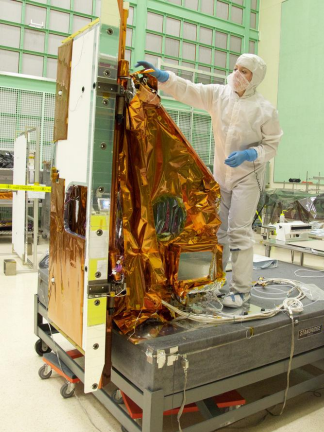
\includegraphics[width=0.7\linewidth]{graficos/TIRS}
			\caption[Construcción del sensor TIRS, desarrollado el (GSFC) Goddard Space Flight Center,
			Greenbelt y por la NASA.]{Construcción del sensor TIRS, desarrollado el (GSFC) Goddard Space Flight Center,
				Greenbelt y por la NASA.
				
				Fuente: \parencite{ldcm-l8}
			}
			\label{fig:TIRS}
			
		\end{figure}
		
		\subsubsection{Sistema Terrestre}
		
		El sistema terrestre de Landsat se encarga del control y administración del satélite Landsat 8  en órbita, así como de la gestión y distribución de los datos transmitidos por el observatorio. El centro de operaciones de misión Landsat, ubicado en Goddard, NASA, envía comandos de software al satélite a través de la red de estaciones terrestres del L8, llamada GNE (Ground Network Element). Esta red cuenta con tres nodos: en Gilmore Creek (Alaska), Svalbard (Noruega), y Sioux Falls (Dakota del Sur), donde se reciben los datos del satélite.
		
		Una vez que los datos son transmitidos desde el observatorio al GNE, son enviados al sistema de procesamiento y archivo de datos (DPAS) ubicado en el EROS Center en Sioux Falls, a través de internet. Desde allí, los datos se archivan, se generan productos científicos del L8 y se ponen a disposición de la comunidad científica a través de un portal de datos \parencite{ldcm-l8}.
		
		\subsubsection{Plataforma del Satélite l8}
		Consta de una serie de subsistemas:
		
		1. Subsistema mecánico.
		
		2. Subsistema de mando y manejo de datos.
		
		3. Subsistema de control de altitud.
		
		4. Subsistema de energía eléctrica.
		
		5. Subsistema de radio frecuencia (RF).
		
		6. Subsistema de propulsión de hidrasina.
		
		7. Subsistema de control térmico.
		
			El panel solar desplegable de 9.75x2.6 metros (32x8.5 pies) genera la energía necesaria para los componentes de la sonda y carga las baterías de níquel-hidruro o níquel-dihidruro (Ni-H2) de la nave, que almacenan una capacidad de 125 amperios-hora. Además, la nave cuenta con un grabador de estado sólido de 3.14 terabits, que proporciona almacenamiento a bordo, y una antena de banda X para transmitir los datos recogidos por los sensores OLI y TIRS. Estos sensores están montados en un banco óptico en la parte frontal de la nave.
		
		La empresa Orbital Science Corporation fue responsable del diseño y fabricación de la plataforma del Landsat 8, así como de la integración de los instrumentos y las pruebas completas de validación \parencite{ldcm-l8}.
	\end{comment}
	\subsection{Programa Satélite Landsat 8}
	
	El Programa Landsat, iniciado en 1972 por la NASA y el USGS, revolucionó el estudio de la Tierra con la serie más extensa de datos satelitales sobre cambios en la superficie terrestre. Actualmente, su octava misión, Landsat 8, incluye el satélite LDCM, equipado con los sensores OLI (Operational Land Imager) y TIRS (Thermal Infrared Sensor). Este satélite sigue trayectorias previas, asegurando la continuidad de los datos. Proporciona imágenes con resolución de hasta 15 metros y cobertura de 170 x 183 km, útiles para estudios de temperatura, áreas costeras y detección de nubes \parencite{ldcm-l8}.
	
	\subsubsection{Plataforma del Satélite l8}
	El Landsat 8 cuenta con múltiples subsistemas (mecánico, control térmico, propulsión, RF, entre otros). Posee un panel solar de 9.75 x 2.6 metros que genera 3750 W y carga baterías de Ni-H2 con 125 Ah de capacidad. También dispone de un grabador de estado sólido de 3.14 Tb y una antena de banda X para transmitir datos captados por los sensores OLI y TIRS \parencite{ldcm-l8}.

	
	\begin{figure}[h!]
		\centering
		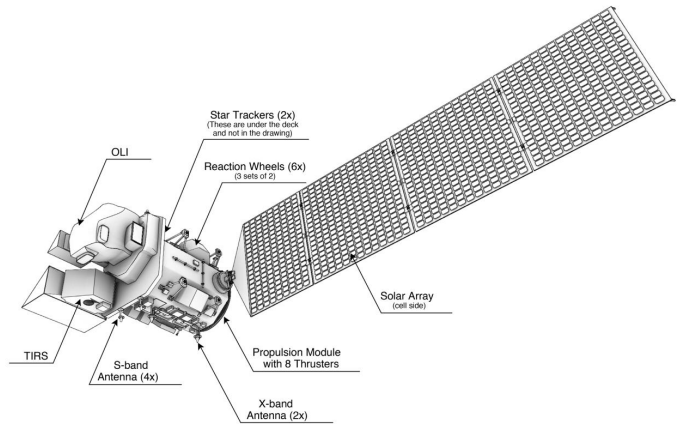
\includegraphics[width=0.7\linewidth]{graficos/l8}
		\caption[Subsistemas de la plataforma L8.]{Subsistemas de la plataforma L8.
			
			Fuente: \parencite{ldcm-l8}
		}
		\label{fig:l8}
		
	\end{figure}

	
	A continuación se presenta una descripción técnica de los productos del L8:
	
	\textbf{Masa:} 2,782 kg (6,113 lbs)
	
	\textbf{Órbita:} Circular a 705 km con una inclinación de 98.2 grados
	
	\textbf{Estabilidad del objetivo:} 6.02 microradianes
	
	\textbf{Almacenamiento de datos:} Grabadora de estado sólido de 3.14 terabits
	
	\textbf{Transmisión de datos:} Banda X, 384 Mbps (en más de dos canales)
	
	\textbf{Propulsión:} 395 kg (870 lbs) de monopropelente de hidracina con 8 propulsores de 22 Newton
	
	\textbf{Vida útil:} 5 años
	
	\begin{comment}
			\subsection{Programa Satélite Landsat 5}
		
		El Landsat 5 fue una de las primeras misiones operacionales del programa Landsat, lanzada en marzo de 1982. Su principal objetivo era monitorear los recursos terrestres mediante imágenes multiespectrales de alta resolución espacial, capturando la radiación solar reflejada desde la superficie de la Tierra. El satélite permaneció en órbita hasta junio de 2013.
		
		El sensor Thematic Mapper (TM) ofrecía una resolución espacial de 30 metros para las bandas visibles y cercanas al infrarrojo, y 120 metros para la banda térmica. Además, su cobertura abarcaba franjas de 185 km de ancho \parencite{landsat5_mission}.
		
		\subsubsection{Sensor Thematic Mapper (TM)}
		
		El sensor TM fue diseñado y construido por el Santa Barbara Research Center (SBRC) de Hughes Aircraft Company. Es un escáner multiespectral mecánico de tipo whiskbroom que trabaja en las regiones visible e infrarroja del espectro electromagnético (EMS). Whiskbroom que emplea espejos móviles para escanear la superficie terrestre en franjas, lo que lo diferencia del sistema pushbroom, que utiliza filas de detectores alineados, capturando la imagen sin partes móviles. Aunque whiskbroom tiene más partes móviles.
		
		El telescopio del TM es del tipo Ritchey-Chrétien, con un diámetro de 44.6 cm. Algunas especificaciones técnicas incluyen una abertura transparente de 41.15 cm, un espejo secundario de 15.7 cm y una longitud focal efectiva de 243.8 cm (f/6).
		
		El instrumento completo mide 2.0 m x 1.1 m x 0.7 m y tiene una masa de 258 kg. Su consumo máximo es de 385 W y utiliza una cuantificación de 8 bits. Aunque fue diseñado para una vida útil de 2 años, logró superar este tiempo, alcanzando una meta de 3 años. Las imágenes obtenidas cubren un área de 185 km por 172 km, con una resolución de 5760 líneas por 6928 píxeles. La transmisión de datos se realiza a una frecuencia de 8215.5 MHz (banda X) con una velocidad de 84.9 Mbit/s (246 MBytes por escena) \parencite{landsat5_mission}.contenidos...
	\end{comment}
	
	\subsection{Programa Satélite Landsat 5}
	
	Lanzado en marzo de 1982, el Landsat 5 tuvo como objetivo monitorear recursos terrestres mediante imágenes multiespectrales de alta resolución. Operó hasta junio de 2013, superando su vida útil inicial de 2 años. Utilizaba el sensor Thematic Mapper (TM), que capturaba imágenes con resolución de 30 metros (bandas visibles e infrarrojas) y 120 metros (banda térmica), cubriendo franjas de 185 km de ancho \parencite{landsat5_mission}.
	
	\subsubsection{Componentes de espacio y hardware}
	
	El Landsat 5 contaba con una matriz solar articulada que generaba 1430 W y dos baterías de NiCd con 100 Ah para la fase de eclipse. Incluía un sistema de propulsión de hidrazina para mantener la órbita y equipamiento avanzado como antena TDRS, GPS y un módulo de banda ancha. Su diseño destacó por la confiabilidad y longevidad, contribuyendo significativamente al monitoreo ambiental global \parencite{landsat5_mission}.
	
	\begin{figure}[h!]
		\centering
		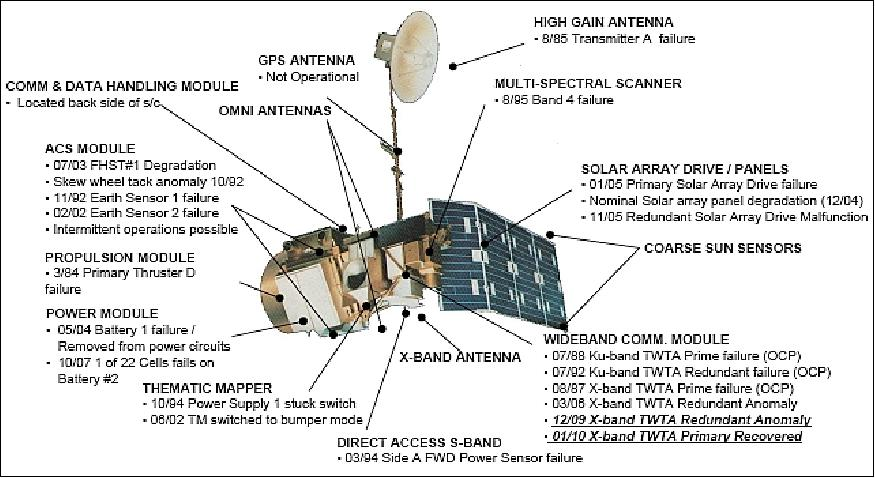
\includegraphics[width=0.7\linewidth]{graficos/L5}
		\caption[Subsistemas de la plataforma L5.]{Subsistemas de la plataforma L5.
			
			Fuente: \parencite{landsat5_mission}
		}
		\label{fig:L5}
		
	\end{figure}

	
	\subsection{Landsat 8 OLI/TIRS Collection 2 Level 1}
	
	Los productos Level 1 Precision Terrain (L1TP) se entregan como números digitales (DN) en un formato entero de 16 bits sin signo, los cuales pueden convertirse en reflectancia o radiancia en la parte superior de la atmósfera (TOA) utilizando los factores de escala radiométrica proporcionados en los archivos de metadatos de cada escena. Además, están corregidos tanto radiométrica como geométricamente. Las Tablas 1 y 2 muestran las referencias y especificaciones de las bandas OLI, respectivamente \parencite{landsat8}.
	
	\begin{table}[h!]
		\centering
		\begin{tabular}{|c|c|c|}
			\hline
			\textbf{Numero de banda} & \textbf{Descripción de banda} &\textbf{Rango de banda (nm)}\\
			\hline
			1  & Coastal Aerosol (Operational Land
			Imager (OLI)) & 435-451\\
			2 & Blue (OLI) & 452-512\\
			3 & Green (OLI) & 533-590 \\
			4 & Red (OLI) & 636-673 \\
			5 & Near-Infrared (NIR) (OLI) & 851-879 \\
			6 & Short Wavelength Infrared (SWIR) 1
			(OLI) & 1566-1651 \\
			7 & SWIR 2 (OLI) & 2107-2294 \\
			8 & Panchromatic (OLI)  & 503-676\\
			9 & Cirrus (OLI)  & 1363-1384 \\
			10 & Thermal Infrared Sensor (TIRS) 1 & 10600-11190 \\
			11 & TIRS 2  & 11500-12510 \\
			
			\hline
		\end{tabular}
		\caption{Referencia de bandas}
		\label{tabla2.1}
	\end{table}
	
	
	
	\begin{table}[h!]
		\centering
		\begin{tabular}{|c|c|c|c|c|}
			\hline
			\textbf{Numero de banda} & \textbf{Identificador} &\textbf{Tipo de dato} & \textbf{Unidad} & \textbf{Rango}\\
			\hline
			1  & B1 & UINT16 &W/(m2 sr um)& [1 - 65535]\\
			2 & B2 & UINT16&W/(m2 sr um)& [1 - 65535]\\
			3 & B3 & UINT16&W/(m2 sr um)& [1 - 65535] \\
			4 & B4 & UINT16&W/(m2 sr um)& [1 - 65535] \\
			5 & B5 & UINT16&W/(m2 sr um)& [1 - 65535] \\
			6 & B6 & UINT16&W/(m2 sr um)& [1 - 65535] \\
			7 & B7 & UINT16 &W/(m2 sr um)& [1 - 65535] \\
			8 & B8  & UINT16&W/(m2 sr um)& [1 - 65535]\\
			9 & B9  & UINT16 &W/(m2 sr um)& [1 - 65535]\\
			\hline
		\end{tabular}
		\caption{Especificaciones de las bandas OLI}
		\label{tabla2.2}
	\end{table}
	
	\begin{table}[h!]
		\centering
		\begin{tabular}{|c|c|c|c|c|}
			\hline
			\textbf{Numero de banda} & \textbf{Identificador} &\textbf{Tipo de dato} & \textbf{Unidad} & \textbf{Rango}\\
			\hline
			10  & B10 & UINT16 &W/(m2 sr um)& [1 - 65535]\\
			11 & B11 & UINT16&W/(m2 sr um)& [1 - 65535]\\
			
			\hline
		\end{tabular}
		\caption{Especificaciones de las bandas TIRS}
		\label{tabla2.3}
	\end{table}
	
	
	%Landsat 8 está equipado con el sensor Operational Land Imager (OLI), que mide en las porciones visibles, del infrarrojo cercano y de onda corta del espectro. Sus imágenes presentan resoluciones espaciales multiespectrales de 30 metros, abarcando una franja de 185 km de ancho, lo que permite cubrir amplias áreas del paisaje terrestre.
	
	%Los productos de reflectancia de superficie del Landsat 8 OLI se generan utilizando el algoritmo Land Surface Reflectance Code (LaSRC) (Versión 1.5.0). La reflectancia de la superficie (una medida sin unidades) calcula la fracción de la radiación solar entrante que se refleja desde la superficie de la Tierra hacia el sensor Landsat. Los algoritmos de reflectancia de la superficie, como LEDAPS y LaSRC, corrigen los efectos de dispersión y absorción variables en el tiempo, espacio y espectro, causados por gases atmosféricos, aerosoles y vapor de agua. Esto es esencial para caracterizar de manera fiable la superficie terrestre  \parencite{usgs_landsat_2024}.
	
	Cada imagen de L1TP se encuentra en un aarchivo independente. Cada banda es un archivo Cloud Optimized GeoTIFF (COG) en escala de grises, los archivos de imagen contenen las etiquetas y claves definidas por la especificación del formato de archivo de imagen con etiquetas geograficas (GeoTIFF), donde GeoTIFF define un conjunto de etiquetas Tagged Image File Format (TIFF), que describen información cartográfica y geodética asociada con imágenes geograficas TIFF. 
	
	\subsection{Landsat Thematic Mapper (TM) Collection 2 Level 1}
	
	Los productos estándar L1TP, que se presentan como números digitales (DN) en un formato entero de 8 bits sin signo, pueden convertirse en reflectancia TOA mediante los factores de escala indicados en los metadatos del producto.
	
	El producto L1TP incluye correcciones radiométricas, geométricas y de precisión, y utiliza un DEM para corregir el error de paralaje causado por el relieve topográfico local. Las Tablas 3 y 4 presentan las referencias y especificaciones de las bandas TM, respectivamente \parencite{landsat8}.
	
	
	\begin{table}[h!]
		\centering
		\begin{tabular}{|c|c|c|}
			\hline
			\textbf{Numero de banda} & \textbf{Descripción de banda} &\textbf{Rango de banda (nm)}\\
			\hline
			1 & Blue (TM) & 450-520\\
			2 & Green (TM) & 520-600 \\
			3 & Red (TM) & 630-669 \\
			4 & Near-Infrared (NIR) (TM) & 760-900 \\
			5 & Short Wavelength Infrared (SWIR) 1
			(TM) & 1550-1750 \\
			6 & Thermal Infrared 1 (TM)& 10400-12500 \\
			7 & SWIR 2 (TM) & 2080-2350 \\
			
			
			\hline
		\end{tabular}
		\caption{Referencia de bandas}
		\label{tabla2.4}
	\end{table}
	
	\begin{table}[h!]
		\centering
		\begin{tabular}{|c|c|c|c|c|}
			\hline
			\textbf{Numero de banda} & \textbf{Identificador} &\textbf{Tipo de dato} & \textbf{Unidad} & \textbf{Rango}\\
			\hline
			1  & B1 & UINT8 &W/(m2 sr um)& [1 - 255]\\
			2 & B2 & UINT8&W/(m2 sr um)& [1 - 255]\\
			3 & B3 & UINT8&W/(m2 sr um)& [1 - 255] \\
			4 & B4 & UINT8&W/(m2 sr um)& [1 - 255] \\
			5 & B5 & UINT8&W/(m2 sr um)& [1 - 255] \\
			6 & B6 & UINT8&W/(m2 sr um)& [1 - 255] \\
			7 & B7 & UINT8 &W/(m2 sr um)& [1 - 255] \\
			\hline
		\end{tabular}
		\caption{Especificaciones de las bandas TM}
		\label{tabla2.5}
	\end{table}
	
	\subsection{Indice espectral}
	Los índices espectrales llegan a ser combinaciones paramétricas de bandas o canales espectrales, estos índices nos ayudan a analizar aspectos territoriales, para el análisis de vegetación, coberturas de agua, coberturas de nieve, proliferación de algas acuáticas, cálculos de niveles de humedad en el terreno, etc \parencite{eos}.
	
	\subsubsection{Índice diferencial normalizado de nieve (NDSI)}
	Al desear identificar la presencia de nieve, los sensores de los satélites incluyen mediciones a 0.66 y 1.6 mm. Al haber transparencia de la atmósfera en estas longitudes de onda, al tiempo que la nieve no es reflectante a 1,6 mm y muy reflectante a 0,66 mm.
	La capa de nieve llega a ser tan brillante como las nubes, esto hace que sea mu complicado diferenciarlas una de otra. Sin embargo, a 1,6 mm, la capa de nieve absorbe la luz solar y es por esa razón aparece representada más oscura que las nubes. Esto permite una distinción efectiva y notoria entre las nubes y los cuerpos de nieve. La imagen, por lo tanto, demuestra la habilidad de separar las nubes de la nieve usando observaciones en estas longitudes de onda. 
	El índice NDSI es una medida de la magnitud relativa de la diferencia de reflectancia entre el rango visible del espectro (verde) y el infrarrojo de onda corta (SWIR). Este índice controla la variación de dos bandas, una de ellas en el infrarrojo cercano o en el infrarrojo de onda corta y la otra en las partes visibles del espectro. Esto es adecuado para el mapeo y análisis de nieve. La nieve es reflectante en el espectro visible y además muy absorbente en el infrarrojo cercano (NIR) o en la parte infrarroja de onda corta del espectro mientras que la mayor parte de la reflectancia de las nubes continúa siendo alta en las mismas partes del espectro, en efecto esto permite una buena separación de la mayoría de las nubes y la nieve \parencite{eos}.
	
	\subsubsection{Fórmula del NDSI}
	La relacion entre las bandas captadas que llegan a componer una imagen de satélite para cuerpos de nieve, tiene la siguiente fórmula.
	
	NDSI = \(\frac{GREEN - SWIR}{GREEN + SWIR}\)
	
	\subsection{Procesamiento de imágenes digitales}
	
	En la actualidad, las imágenes constituyen un lenguaje en sí mismas, puesto que las imágenes llegan a transmitir distintos tipos de información. Por esto, es muy necesario contar con un soporte para la representación digital de las imágenes que nos permita luego modificar el mismo, esto con el fin de modificar el contenido visual, simbólico y obtener la información necesaria \parencite{jahne2005digital}.

	
	Según \parencite{gonzalez2008digital}, una imagen puede definirse como una función bidimensional f(x,y), donde x e y son coordenadas espaciales, y la amplitud de f en cualquier punto (x,y) se denomina intensidad o nivel de gris de la imagen en ese punto. Cuando x, y y los valores de intensidad de f son cantidades discretas y finitas, llamamos a la imagen una imagen digital. En el campo de las imágenes digitales, esto se refiere al procesamiento de estas mediante una computadora digital. Una imagen digital se compone de un número finito de elementos, cada uno con una ubicación y un valor específico; estos elementos se denominan comúnmente píxeles.
	
	Además la visión humana, uno de nuestros sentidos más avanzados, está limitada a la percepción de la banda visual del espectro electromagnético (EM). Sin embargo, las máquinas de imágenes pueden abarcar casi todo el espectro EM, desde ondas gamma hasta ondas de radio, y generar imágenes a partir de fuentes no convencionales para el ser humano, como el ultrasonido, la microscopía electrónica e imágenes generadas por computadora.
	
	El procesamiento digital de imágenes cubre un campo amplio y diverso de aplicaciones. Además, existen campos como la visión artificial, cuyo objetivo es utilizar computadoras para emular la visión humana, incluyendo el aprendizaje, la capacidad de hacer inferencias y tomar decisiones basadas en entradas visuales. Esta área es una rama de la inteligencia artificial, destinada a imitar la inteligencia humana.
	
	%Una imagen puede describirse como una función bidimensional f(x,y), donde x e y representan las coordenadas espaciales y la amplitud de f en cada punto indica la intensidad o nivel de gris. Cuando x, y y los valores de intensidad de f son discretos y finitos, la imagen es digital y está compuesta por píxeles, cada uno con una posición y valor específicos. Aunque la visión humana solo percibe el espectro visible, las máquinas pueden capturar imágenes a lo largo de casi todo el espectro electromagnético, desde ondas gamma hasta radiofrecuencia, utilizando fuentes no habituales como ultrasonido o microscopía electrónica. El procesamiento digital de imágenes abarca aplicaciones amplias y variadas, incluyendo la visión artificial, un campo de la inteligencia artificial que busca replicar la visión humana en las computadoras, permitiéndoles interpretar y actuar sobre información visual, emulando capacidades como el aprendizaje y la toma de decisiones.
	
	
	\subsubsection{Formación de una imagen digital}
	
	La mayoría de las imágenes que nos interesan se generan mediante la combinación de una fuente de iluminación y la reflexión o absorción de energía de esa fuente por los elementos de la escena captada. Por ejemplo, la iluminación puede provenir de una fuente electromagnética, como radar, infrarrojos o rayos X, pero también podría originarse de fuentes menos tradicionales, como el ultrasonido. De manera similar, los objetos podrían ser familiares o incluso moléculas, formaciones rocosas, etc. Dependiendo de la fuente, la energía de iluminación se refleja desde los objetos o se transmite a través de ellos \parencite{gonzalez2008digital}.
	
	\begin{figure}[h!]
		\centering
		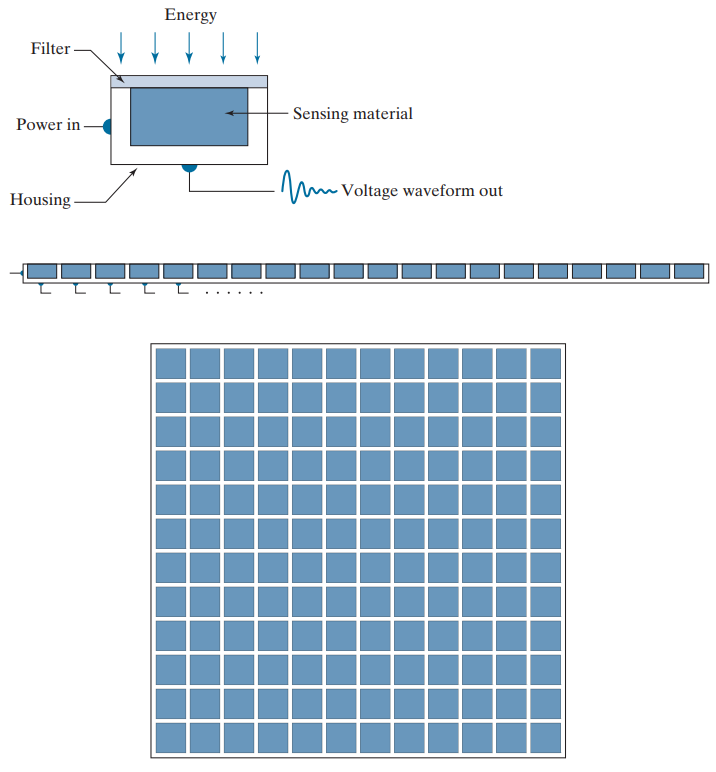
\includegraphics[width=0.7\linewidth]{graficos/sensorImagen}
		\caption[Modélo basico de un sensor para adquirir imágenes.]{Modélo basico de un sensor para adquirir imágenes.
			
			Fuente: \parencite{landsat5_mission}
		}
		\label{fig:sensorImagen}
		
	\end{figure}
	
	Como menciona \parencite{gonzalez2008digital}, en la Figura \ref{fig:sensorImagen} se muestran las tres disposiciones principales de sensores utilizados para transformar la energía incidente en imágenes digitales. La idea es simple: la energía entrante se convierte en un voltaje mediante una combinación de la energía eléctrica de entrada y el material del sensor, que responde al tipo de energía que se detecta. La forma de onda del voltaje de salida es la respuesta del sensor y se obtiene una cantidad digital al digitalizar esa respuesta. Un sensor conocido de este tipo es el fotodiodo, que está construido con materiales de silicio y cuya salida es un voltaje proporcional a la luz. El uso de un filtro delante del sensor mejora su selectividad; por ejemplo, un filtro óptico de transmisión verde favorece la luz en la banda verde del espectro de color. Como consecuencia, la salida del sensor sería más fuerte para la luz verde que para otros componentes de la luz visible.
	
	Para generar una imagen 2D utilizando un único elemento sensor, debe haber desplazamientos relativos en las direcciones x e y entre el sensor y el área que se va a fotografiar. La salida de los sensores se procesa mediante algoritmos de reconstrucción cuyo objetivo es transformar los datos detectados en imágenes transversales.
	
	Como se mencionó anteriormente, una imagen se denota mediante funciones bidimensionales de la forma f(x,y). El valor f en las coordenadas espaciales (x, y) es una cantidad escalar cuyo significado físico está determinado por la fuente de la imagen y cuyos valores son proporcionales a la energía irradiada por una fuente física (por ejemplo, ondas electromagnéticas). Como consecuencia, f(x,y) debe ser no negativo y finito.
	
	\begin{equation}
		\label{eq:img1}
		0 \leq f(x,y) < \infty
	\end{equation}
	
	La función $f(x,y)$ se caracteriza por dos componentes: (1) la cantidad de iluminación de la fuente incidente sobre la escena que se está observando, y (2) la cantidad de luz reflejada por los objetos en la escena. Estos se denominan componentes de iluminación y reflactancia, y se denotan por $i(x,y)$ y $r(x,y)$ respectivamente. Las dos funciones se combinan como un producto para formar $f(x,y)$
	
	\begin{equation}
		\label{eq:img2}
		f(x,y) = i(x,y)r(x,y)
	\end{equation}
	Donde:
	
	\begin{equation}
		\label{eq:img3}
		0 \leq i(x,y) < \infty
	\end{equation}

	y
	
	\begin{equation}
		\label{eq:img4}
		0 \leq r(x,y) < \infty
	\end{equation}
	
	Por lo tanto, la reflectacia está limitada por 0 (absorción total) y 1 (reflctancia total). La naturaleza de i(x,y) está determinada por la fuente de iluminación y r(x,y) está determinada por las caracteristicas de los objetos representados en la imagen \parencite{gonzalez2008digital}.
	
	\begin{figure}[h!]
		\centering
		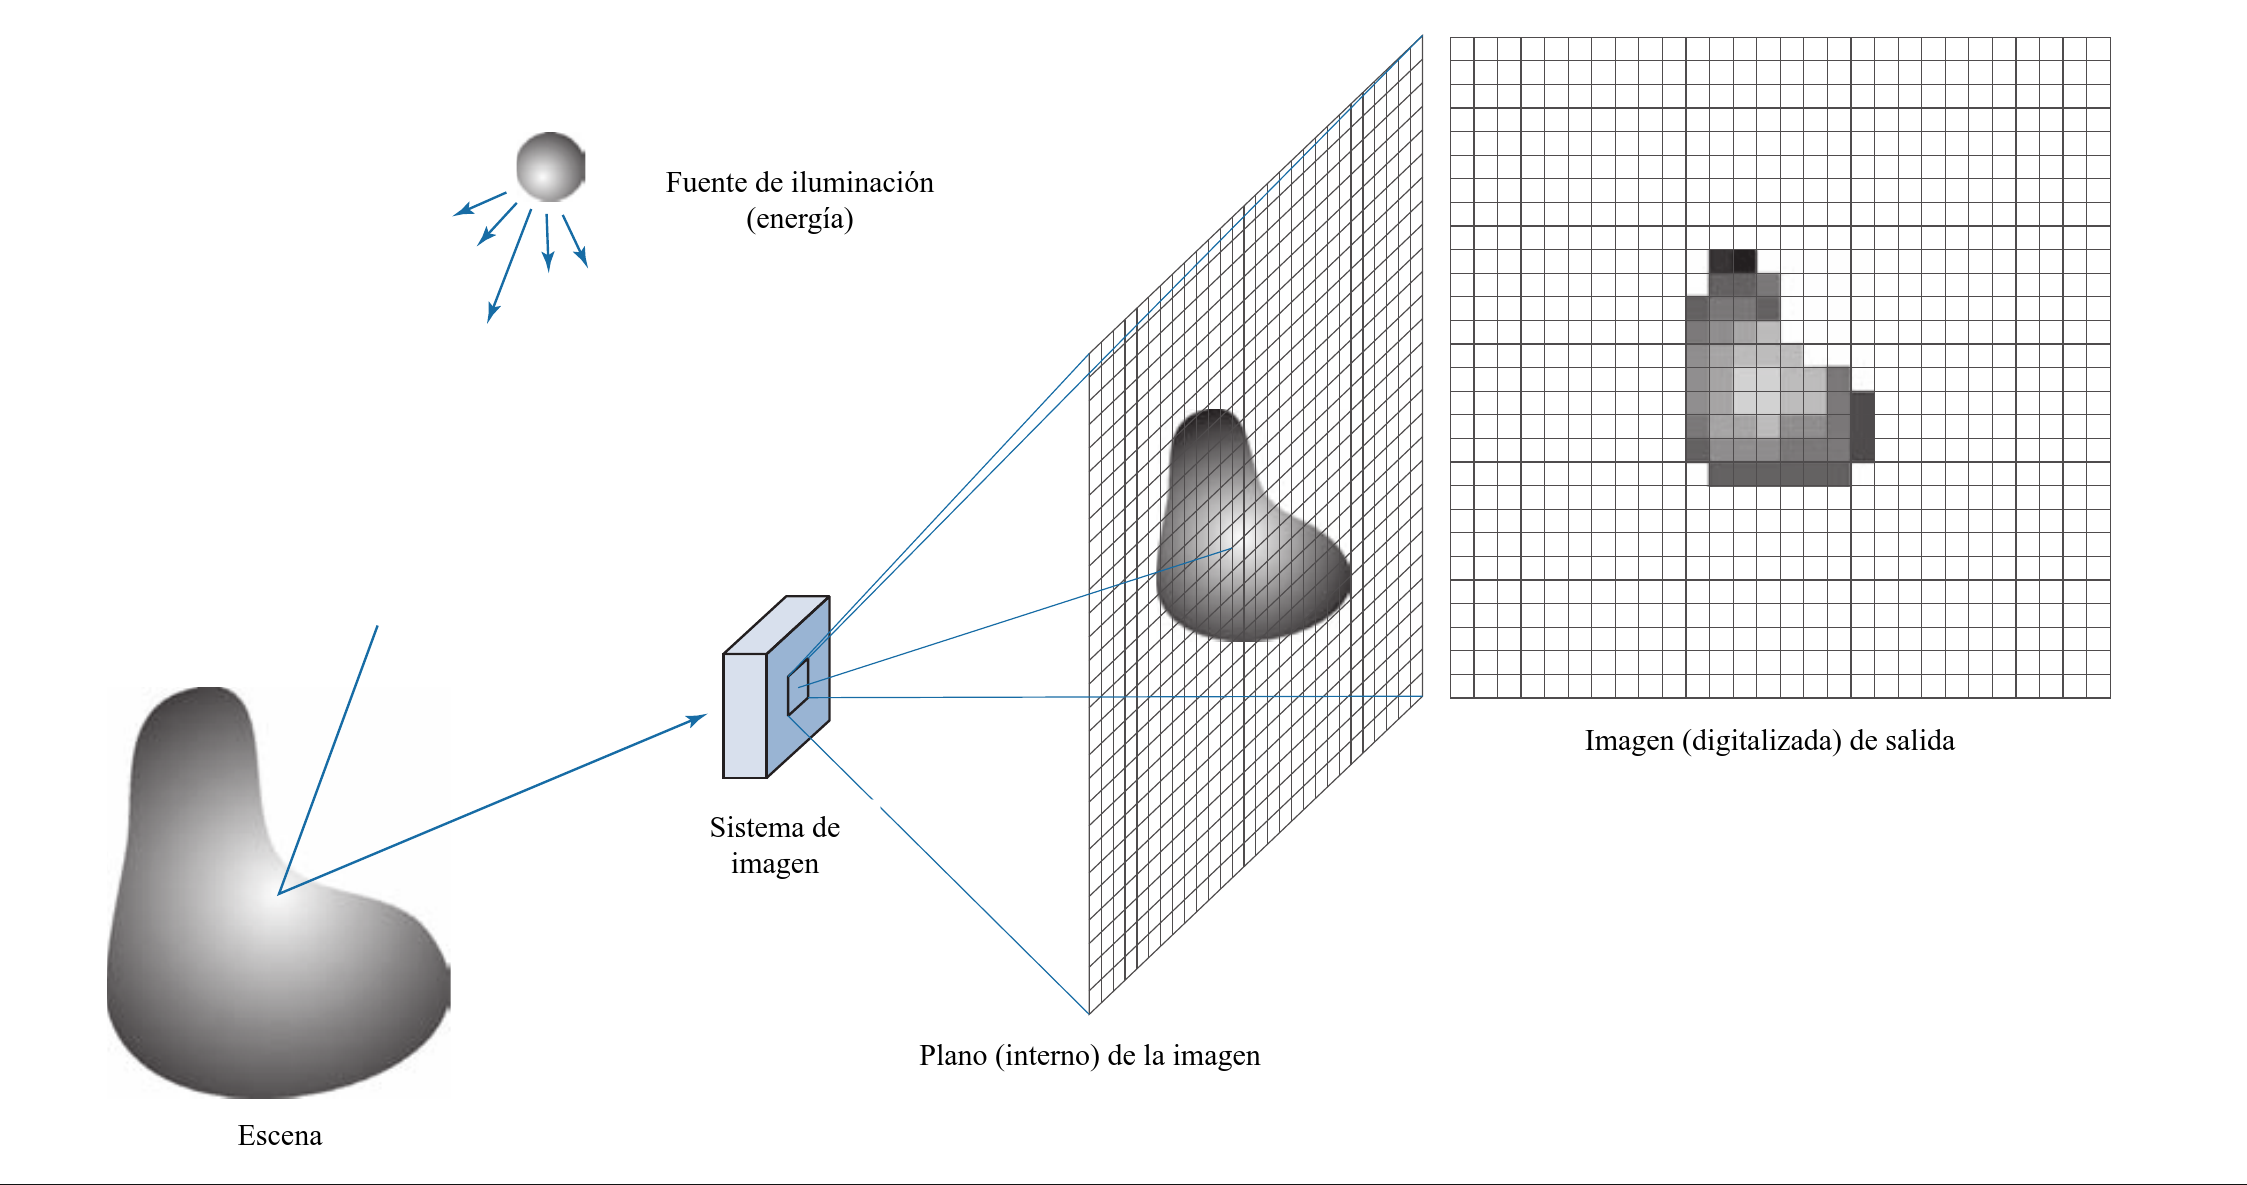
\includegraphics[width=0.8\linewidth]{graficos/drawio}
		\caption[Ejemplo de adquisición y formación de una imagen digital]{Ejemplo de adquisición y formación de una imagen digital: Fuente de iluminación (energía). (b) Una escena. (c) Sistema de
			imágenes. (d) Proyección de la escena sobre el plano de la imagen. (e) Imagen digitalizada.
			
			Fuente: \parencite{gonzalez2008digital}}
		\label{fig:drawio}
	\end{figure}
	
	Un ejemplo de adquisición de imágenes digitales. (a) Fuente de iluminación (energía). (b) Una escena. (c) Sistema de
	imágenes. (d) Proyección de la escena sobre el plano de la imagen. (e) Imagen digitalizada.
	\begin{comment}
	
	\subsubsection{Representación de una imagen digital}
	
	Una imagen digital se representa mediante una matriz numérica, cada elemento de la matriz viene a ser un pixel de la imagen, esta representación numérica es utilizada para el procesamiento computacional, pues es una representación cuantitativa de la imagen.
	
	Una imagen en escala de grises puede ser representada por una matriz bidimensional MXN, sin embargo, las imágenes también pueden ser representadas por una matriz tridimensional conformada por altura, ancho y profundidad, este último conformado por el número de canales de color que contenga la imagen.  
	
	Un claro ejemplo de esto son las imágenes RGB, los cuales contienen 3 canales (rojo, verde y azul), cada canal está formada por una matriz bidimensional, por consiguiente la imagen RGB está conformada por 3 matrices bidimensionales, sucede lo mismo con las imágenes multiespectrales, quienes contienen más de 3 canales \parencite{udacity2019colorimages}.
	
	
	
	: compone tres bandas fundamentales, rojo (λ = 0.6 - 0.7 μm), verde (λ = 0.5 - 0.6 μm) y azul (λ = 0.4 - 0.5 μm), además esta porción del espectro es el rango completo de la energía electromagnética, al cual es sensible al ojo humano (RABOLLI y otros, 2019, pág. 17).
	
	
	Infrarrojo cercano (NIR) que componen de longitudes de onda que varían en el rango de (de λ 0.7 a 1.3 μm) esta porción del espectro permite discriminar masas vegetales asi como las concentraciones de humedad (RABOLLI y otros, 2019, pág. 17).
	Infrarrojo medio (MIR) que componen de longitudes de onda que varían en el rango de (λ de 1.3 a 8 μm): Se tiene la banda del infrarrojo de onda corta (SWIR) (λ =0.5 - 0.6 μm), se emplea para hallar el contenido de humedad en la vegetación o en los suelos. Así mismo, se tiene la banda de infrarrojo medio IRM (aprox. 3.7 μm), decisivo para localización de lugares con alta temperatura (RABOLLI y otros, 2019, pág. 17).
	Infrarrojo lejano o térmico (TIR) que componen de longitudes de onda que varían en el rango de (λ de 8 a 14 μm): Esta banda se emplea para localizar el calor proveniente de gran parte de las cubiertas terrestres (RABOLLI y otros, 2019, pág. 17).
	
	
	%Figura 2.3
	\begin{figure}[htb]
		\centering
		\begin{subfigure}{0.4\linewidth}
			\centering
			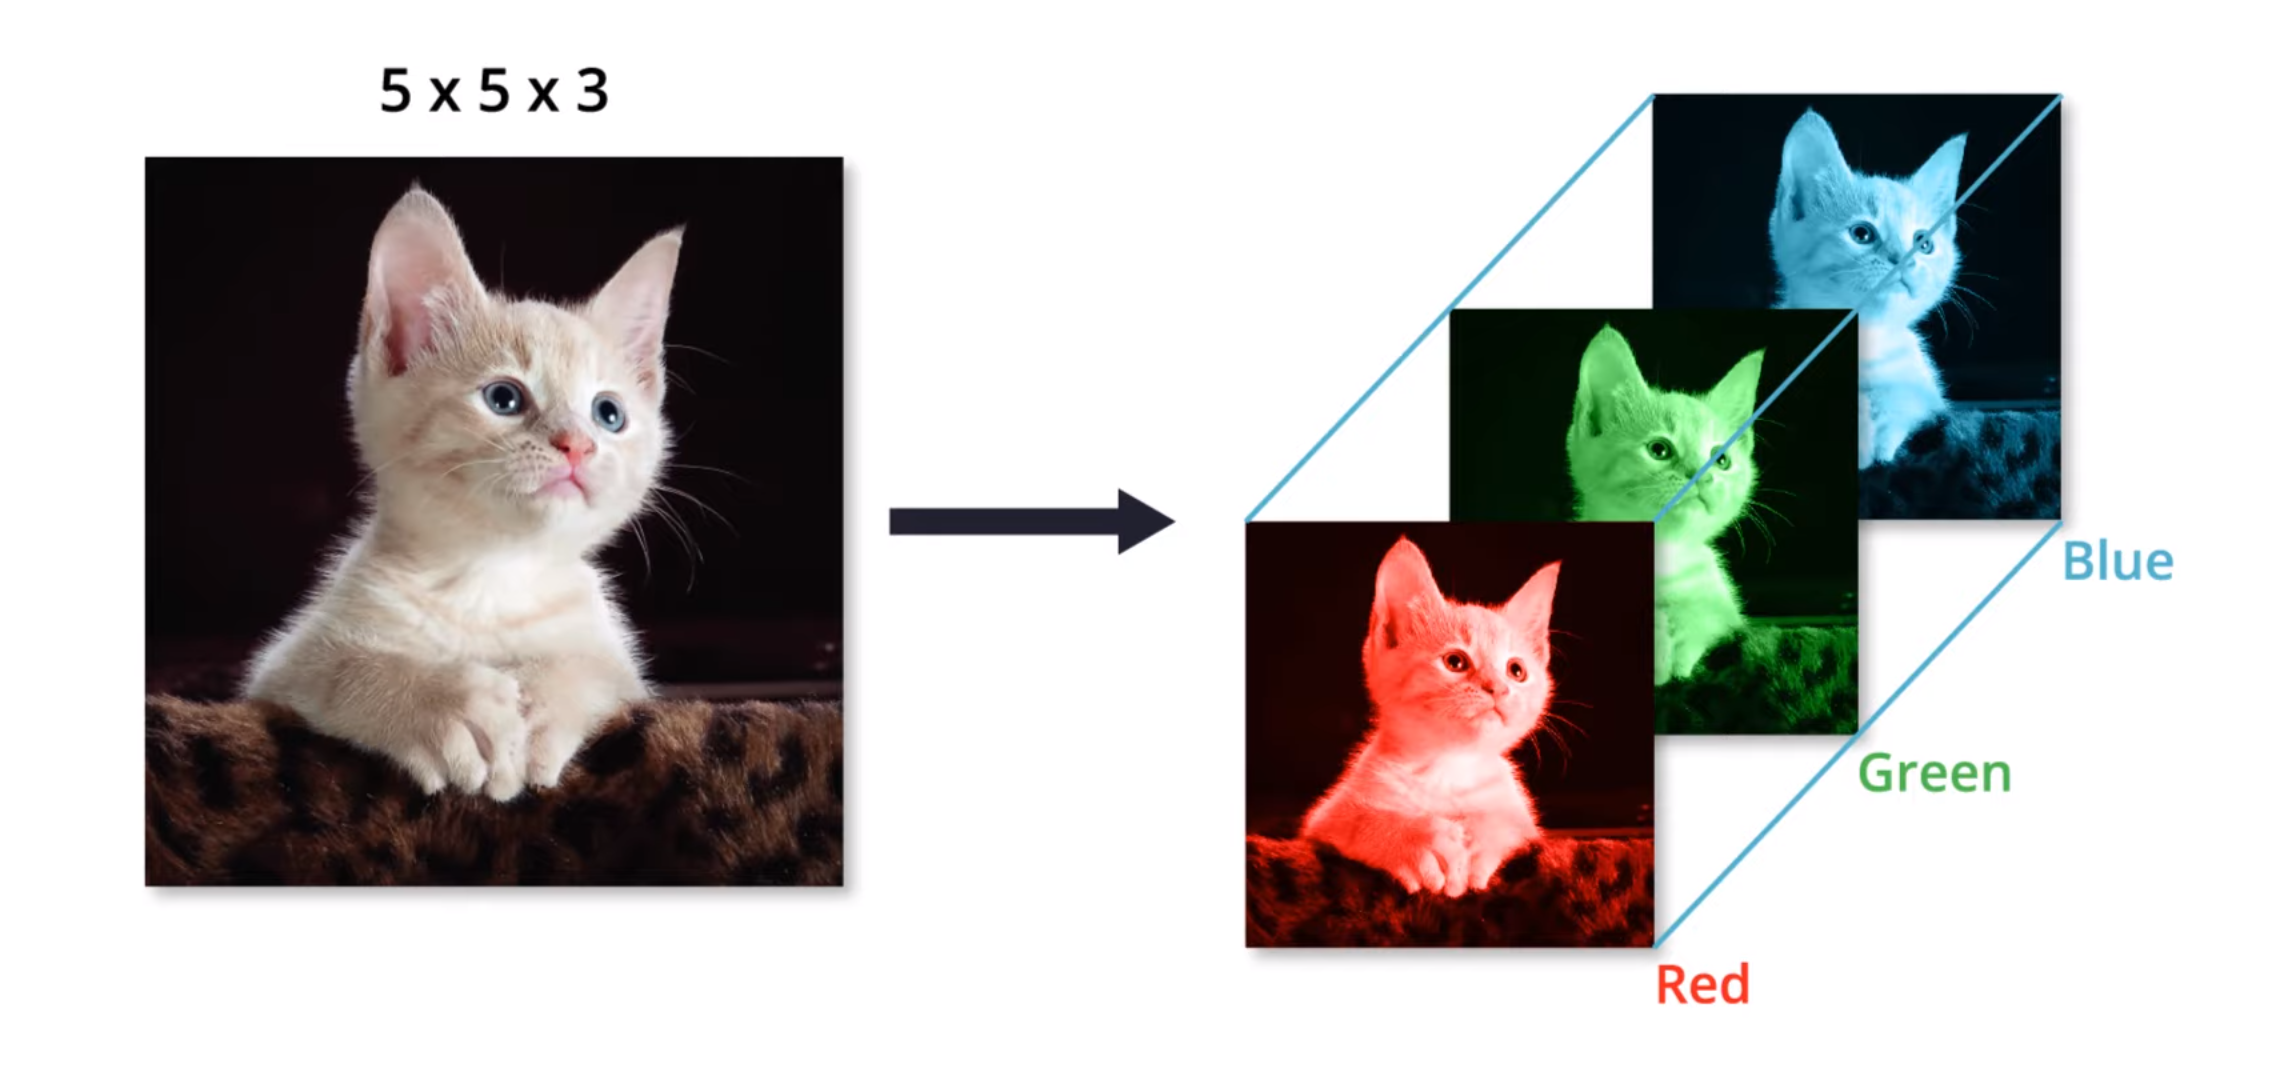
\includegraphics[width=\linewidth]{graficos/RGB_1.png}
			\caption{Canales RGB}
			\label{fig:canales}
		\end{subfigure}
		\hfill
		\begin{subfigure}{0.4\linewidth}
			\centering
			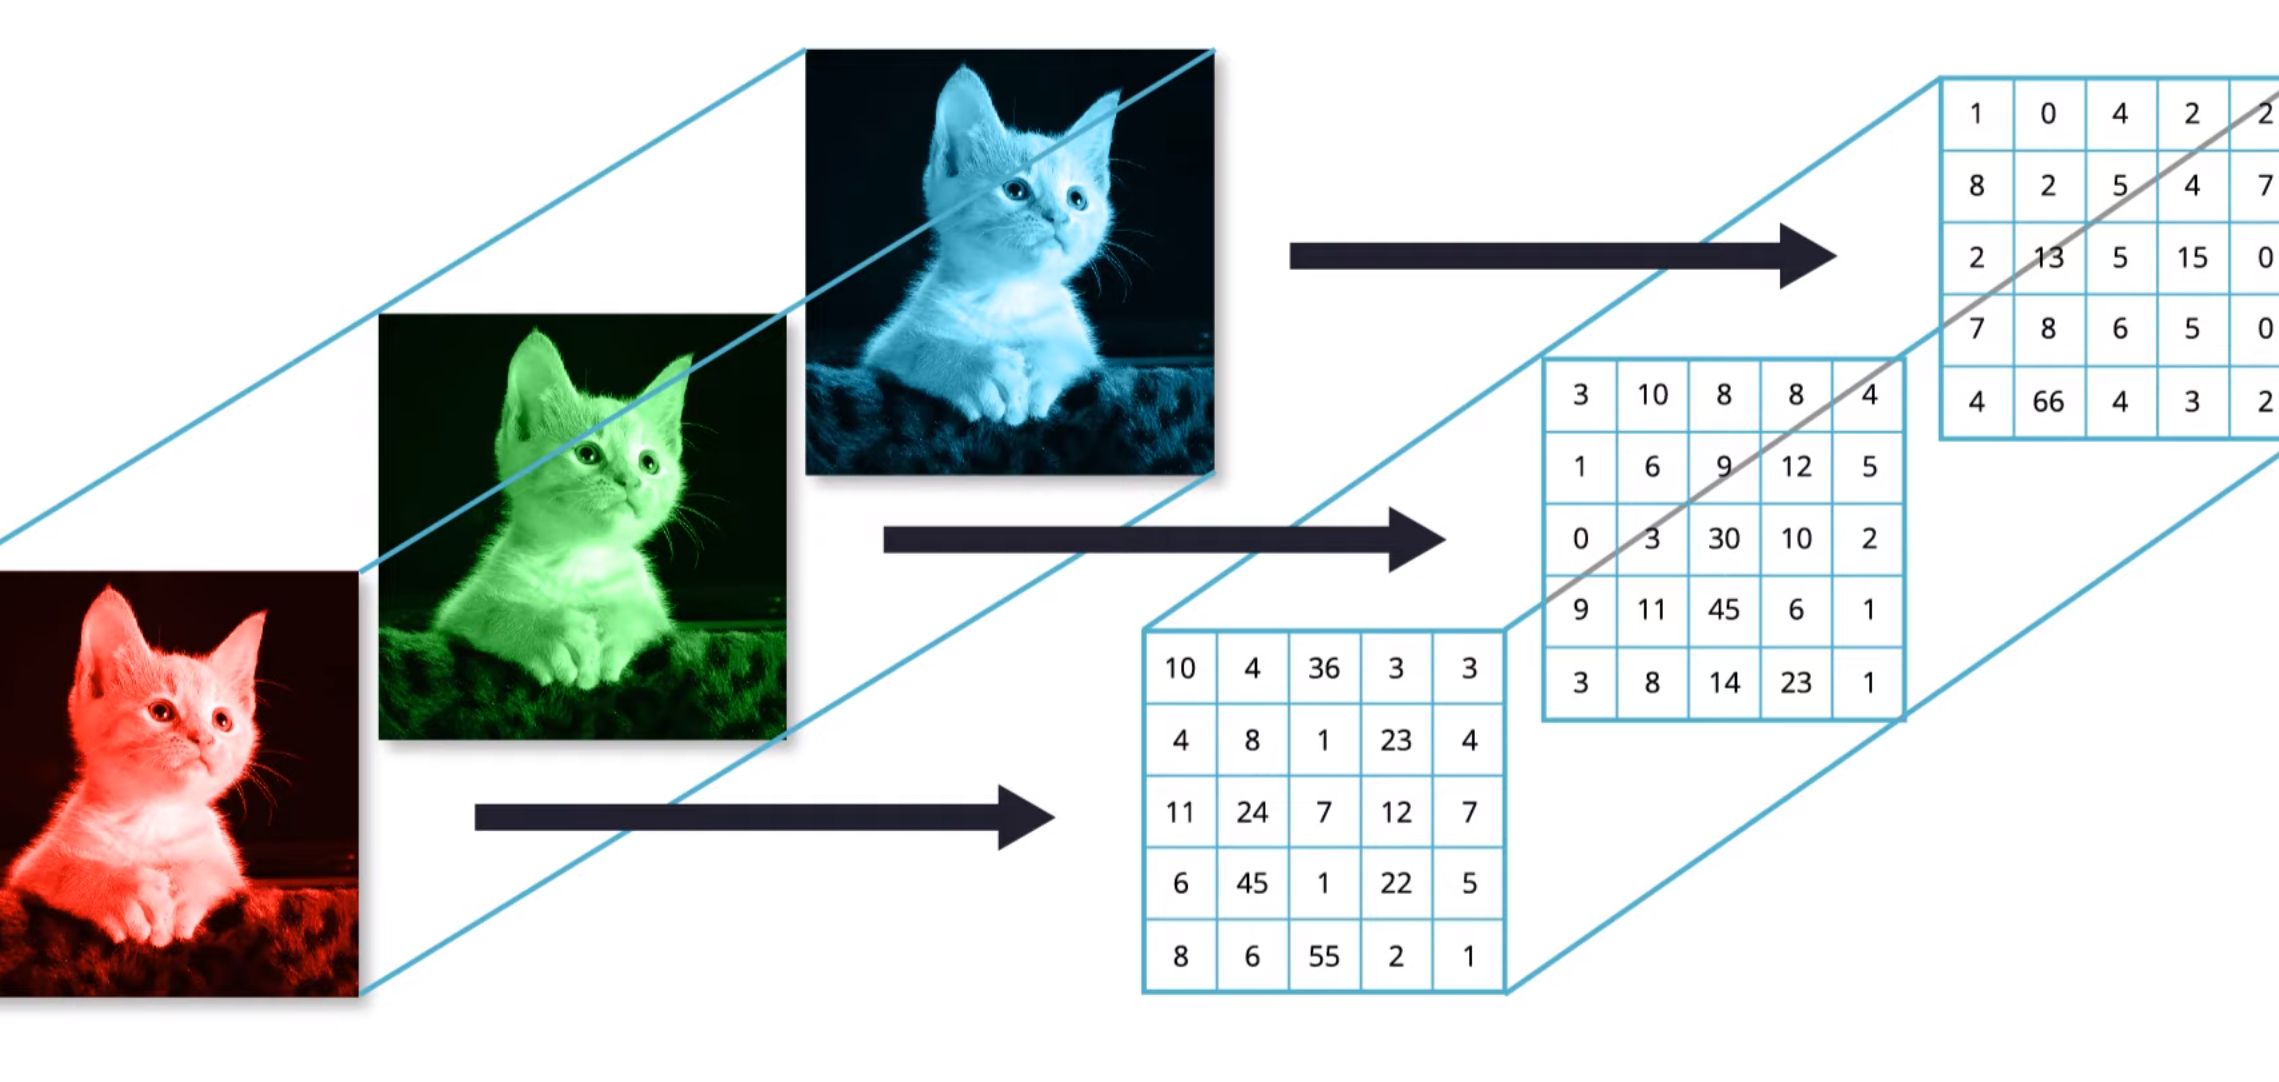
\includegraphics[width=\linewidth]{graficos/RGB_2.png}
			\caption{Matrices bidimensionales}
			\label{fig:matbidi}
		\end{subfigure}
		\hfill
		\begin{subfigure}{0.4\linewidth}
			\centering
			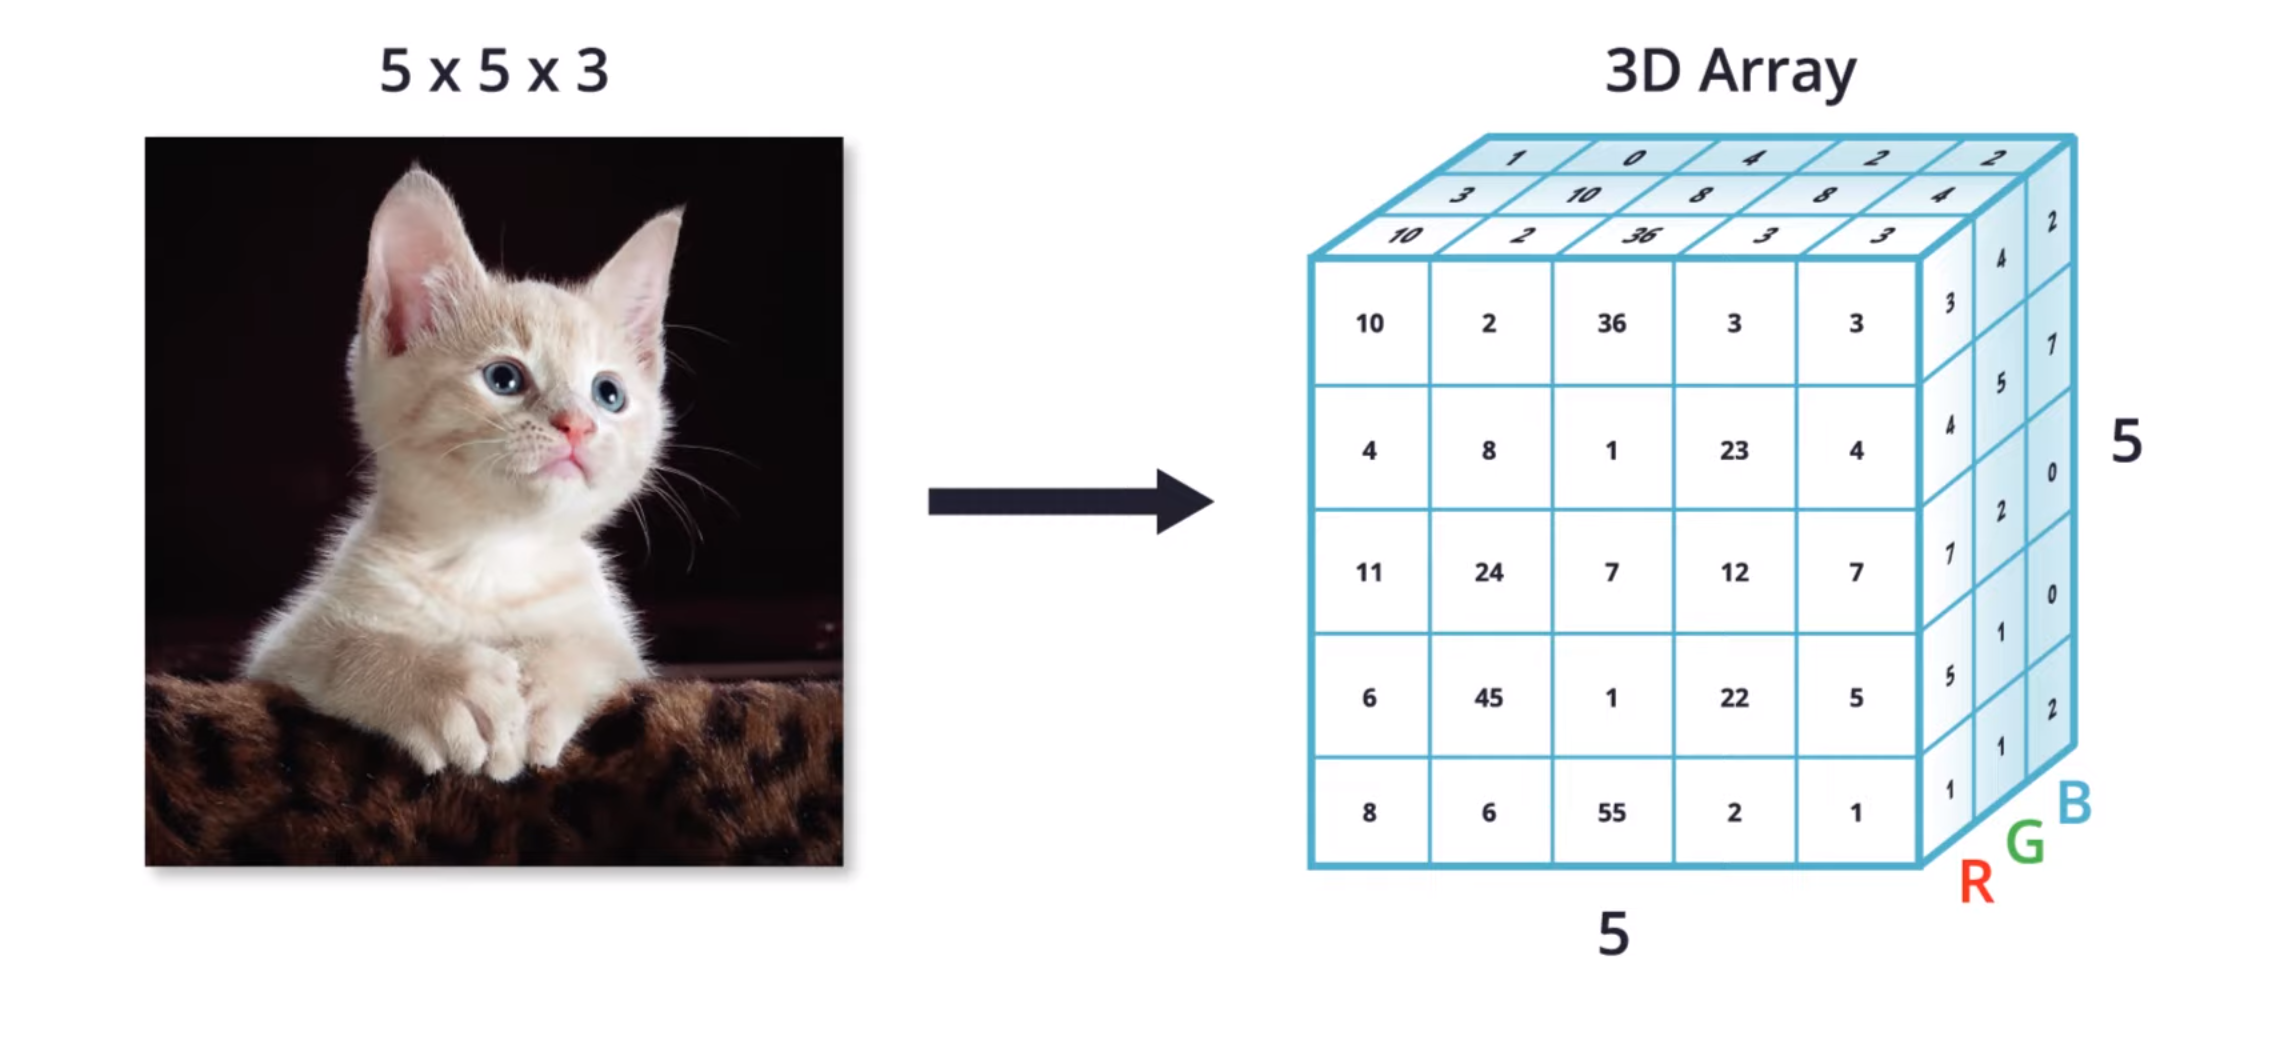
\includegraphics[width=\linewidth]{graficos/RGB_3.png}
			\caption{Matriz tridimensional}
			\label{fig:mattri}
		\end{subfigure}
		\caption[Representación de una imagen RGB]{Representación de una imagen RGB.
			
		Fuente: \parencite{udacity2019colorimages}
		}
		\label{fig:rgb}
	\end{figure}
	
	\end{comment}
	
	\subsection{Deep Learning}
	
	La inteligencia artificial (IA) se ocupa de construir sistemas que simulan comportamientos inteligentes. Dentro de la IA, el aprendizaje automático (Machine Learning) es un subconjunto que ajusta modelos matemáticos a datos observados para tomar decisiones. El aprendizaje profundo (Deep Learning) es un tipo de aprendizaje automático avanzado; sus redes profundas son hoy en día los modelos más potentes \parencite{prince2023understanding}.
	
	Es común usar algoritmos de procesamiento de lenguaje natural para traducir texto, visión artificial para analizar imágenes o asistentes digitales con reconocimiento de voz, esto promete transformar nuestro mundo, aunque no todos los efectos serán positivos.
	
	\begin{figure}[h!]
		\centering
		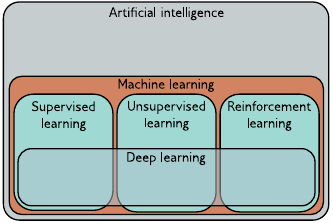
\includegraphics[width=0.7\linewidth]{graficos/deeplearning}
		\caption[Subconjuntos de la inteligencia artificial.]{El Machine Learning viene ser un área de la IA, se puede dividir en aprendizaje supervisado, aprendizaje no supervizado y aprendizaje de refuerzo. El deep learning contribuye a cada una de estas tareas.
			
			Fuente: \parencite{prince2023understanding}
			}
		\label{fig:deeplearning}
	\end{figure}
	
	
	
	\subsection{Estructura de entradas y salidas}
	
	En la Figura \ref{fig:imagen_dl} se puede observar que, en cada caso, hay una entrada significativa del mundo real, ya sea una oración, un archivo de sonido, una imagen, etc. Esta entrada se codifica como un vector de números, el cual forma la entrada del modelo. El modelo asigna esta entrada a un vector de salida, que luego se traduce nuevamente en una predicción significativa del mundo real.
	
	Por ahora, nos centramos en las entradas y salidas, tratando el modelo como una "caja negra" que recibe un vector de números y devuelve otro.
	
	La entrada es un vector de longitud fija que contiene valores que caracterizan una propiedad. Por ejemplo, la Figura \ref{fig:imagen_dl}a representa un modelo de clasificación binaria multivariante para la segmentación semántica. Aquí, a cada píxel de una imagen de entrada se le asigna una etiqueta binaria que indica si pertenece a una vaca o al fondo. La Figura \ref{fig:imagen_dl}b muestra un modelo de regresión multivariante, donde la entrada es una imagen de una escena callejera y la salida es la profundidad en cada píxel.
	
	En ambos casos, la salida es de alta dimensión y estructurada. Sin embargo, esta estructura está estrechamente ligada a la entrada, lo cual se puede explotar; si un píxel está etiquetado como "vaca", es probable que un píxel vecino con valores RGB similares tenga la misma etiqueta.
	
	Las Figuras \ref{fig:imagen_dl}c–e representan tres modelos donde la salida tiene una estructura compleja que no está tan estrechamente ligada a la entrada. La Figura \ref{fig:imagen_dl}c muestra un modelo donde la entrada es un archivo de audio y la salida son las palabras transcritas de ese archivo. La Figura \ref{fig:imagen_dl}d representa un modelo de traducción, en el cual la entrada es un texto en inglés y la salida es su traducción al francés. La Figura \ref{fig:imagen_dl}e muestra una tarea muy desafiante: la entrada es un texto descriptivo, y el modelo debe generar una imagen que coincida con esa descripción \parencite{prince2023understanding}.
	
	\begin{figure}[h!]
		\centering
		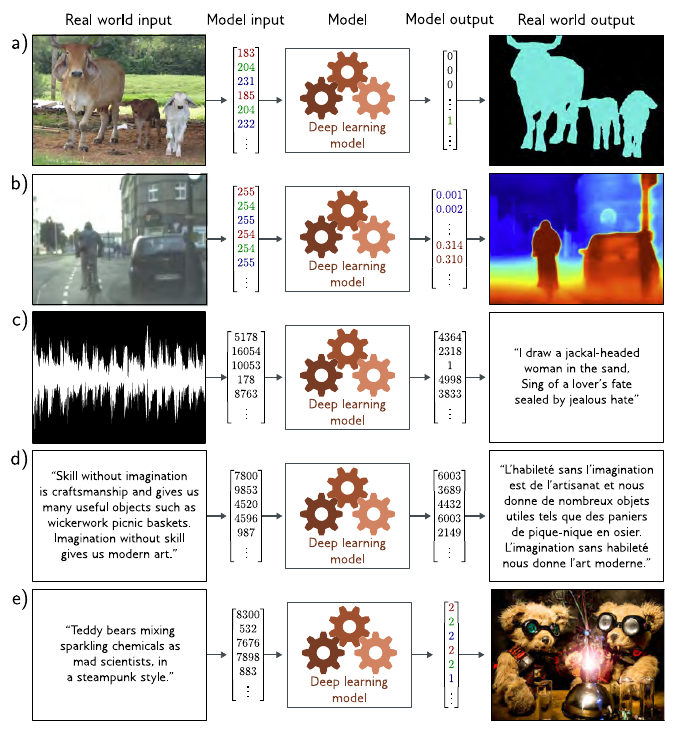
\includegraphics[width=0.7\linewidth]{graficos/imagen_dl}
		\caption[Tareas de aprendizaje supervisado con salidas estructuradas.]{Tareas de aprendizaje supervisado con salidas estructuradas.
			
			Fuente: \parencite{prince2023understanding}
		}
		\label{fig:imagen_dl}
	\end{figure}
	
	\subsection{Aprendizaje Supervizado}
	
	%Hasta ahora se ha tratado el modelo de aprendizaje autoático como si fuera una caja negra el cual toma un vector de entrada y devulve un vector de salida. ¿Pero que hay exactamente en esa caja negra? Considre un modelo para poder predecir la altura de un niño a partir de su edad Fig. El modelo de aprendizaje automatico es una ecuación matemática que describe como varia la altura promedio en función a la edad el cuall esta carecteriza por la curva de color cian, cuando pasamos la edad por esta ecuación devuelve la altura. Por ejemplo si la edad es 11 años, entonces predecmos que la altura será 145 cm. 
	%Más precisamente, el modelo representa una familia de ecuaciones que asigna la entrada a la salida(Una familia de diferentes curvas cian). La ecuación particular se elige utilizando datos de entrenamiento (pares de datos de entrada/salida) en la figura estos pares estan representados por los puntos naranjas y podemos ver que el modelo (linea cian) describe estos datos de manera rasonable. Cuando hablamos de entrenamuento o ajuste de un modelo, nos referimos a que buscamos en la familia de posibes ecuaciones (posibles curvas cian) que relaciona la entrada con la salida para encontrar la que describe los datos de entrenamiento con mayor presición .
	%De ello se deduce que los modelos de la figura requieren pares de entrada/salida etiquetados para el entrenamiento. Pr ejemplo, en la segmentación semantica de vacas requiere una gran catidad de imagenes de vacas, en los cuales un experto humano hubiera identificado el tipo de animal de cada imagen. estos pares de entrada/salida asumen el papel de un profesor o supervisor del proceso de entrenamiento. y esto da lugar al término de aprendizaje supervizado. 
	%El modelo no es mas que una ecuación matematica, CUANDO LAS ENTRADAS PASAN por esta ecuación, esta calcula la salida, lo que se denomina inferencia. La ecuación del modelo tambien contiene parametros, Diferentes valores de los parametros cambian el resultado del calculo; La ecuación del modelo describe una familia de posibles relaciones entre entradas y salidas y los parametros determinan la relación correcta.
	%Para hacer la predicción, necesitamos un modelo f[x] que tome la entrada "x" y devueva la salida "y", dijimos que el modelo tambien contien parametros "p" entonces la elección de los parametros determina l arelación concreta entre la entrada y salida. por lo que en realidad deberiamos escribir Y=f[x,p]
	%Cuando se habla de aprender o entrenar un modelo, quiere decir que se trata de encontrar los parametros que permitan relizar predicciones de salida razonables a partir de la entrada.
	%Aprendenmos estos parametros a partir de datos de entrenamiento, el objetivo es seleccionar parámetros que asignen cada entrada de entrenamiento a su salida asignada lo más fielmente posible.  
	%Cuantificamos el grado de desajuste en esta asignación con la perdida L, este es un valor escalar que resume cuan mal el modelo predice las salidas a partir de sus entradas correspondientes para los parametros p, se puede tratar la perdida como L[p], entonces cuando se entrena un modelo se busca los parametros p que minimizen esta función de perdida. p = argmin[L[p]] Si la perdida de entrenamiento despues de la minimización es pequeña, entonces se encontro los parametros del modelo que predicen con presición los resultados de entrenamiento Yi a partir de los datos de entrada de entrenamiento Xi. DEspués de evaluar el modelo, ahora se debe evaluar su rendimiento ejecutando el modelo con un dato de prueba, para ver que tan bien se genraliza a ejemplos que no obserbó durante el entrenamiento. 
	
	En la Figura \ref{fig:añovsedad}, se observa un modelo de aprendizaje automático tratado como una "caja negra" que recibe un vector de entrada y produce un vector de salida. Ahora bien, ¿qué sucede dentro de esta caja? Imaginemos un modelo que predice la altura de un niño a partir de su edad. El modelo es una ecuación matemática que muestra cómo la altura promedio varía según la edad, representada por una curva en color cian. Así, si se ingresa una edad, el modelo devuelve una altura; por ejemplo, a los 10 años se predice una altura de 139 cms.
	
	Más específicamente, el modelo pertenece a una familia de ecuaciones que mapea la entrada a la salida (una serie de curvas en cian). La ecuación particular se selecciona mediante datos de entrenamiento, que consisten en pares de datos de entrada y salida (marcados en naranja en la figura), y el modelo ajusta esta curva para que represente con precisión estos datos. Este ajuste se conoce como “entrenar el modelo” y se refiere a encontrar, en esta familia de ecuaciones, la que mejor describe los datos de entrenamiento.
	
	En segmentación semántica, como el ejemplo de las vacas, se necesitan imágenes etiquetadas por un humano, lo cual se conoce como aprendizaje supervisado. Aquí, el modelo se comporta como una ecuación matemática donde al ingresar datos, se calculan resultados, proceso llamado “inferencia”. La ecuación tiene parámetros que definen la relación entre entrada y salida, los cuales se afinan durante el entrenamiento. Para hacer predicciones, el modelo utiliza una función $f[x]$ que toma la entrada $x$ y devuelve la salida $y$, donde los parámetros $\phi$ determinan la relación precisa.
	
	Durante el entrenamiento, el modelo ajusta los parámetros para que las predicciones se acerquen lo más posible a las salidas reales, minimizando una función de pérdida $L[\phi]$. La minimización de esta pérdida permite encontrar los mejores parámetros, haciendo que el modelo sea preciso en las predicciones. Después de entrenarlo, se evalúa su rendimiento utilizando un conjunto de prueba, midiendo así su capacidad para generalizarse a datos nuevos no vistos durante el entrenamiento \parencite{prince2023understanding}.
	
	\begin{figure}[h!]
		\centering
		\includegraphics[width=0.7\linewidth]{graficos/añovsedad}
		\caption[Modelo representativo de datos de entrenamiento, entrada/salida.]{El modelo representa una familia de relaciones
			que relacionan la entrada (edad del niño) con la salida (altura del niño). La relación
			en particular se elige utilizando datos de entrenamiento, que consisten en pares de entrada/salida
			(puntos naranjas). Cuando entrenamos el modelo, buscamos entre las posibles relaciones una que describa bien los datos. Aquí, el modelo entrenado es la curva
			cian y se puede utilizar para calcular la altura para cualquier edad. Fuente: \parencite{prince2023understanding}
		}
		\label{fig:añovsedad}
	\end{figure}
	
	\subsection{Función de perdida}
	
	La función de pérdida o función de coste, mencionada anteriormente, mide el desajuste entre el modelo y el conjunto de datos de entrenamiento, el cual está compuesto por pares de datos de entrada/salida $[xi, yi]$ como se observa en la Figura \ref{fig:desajuste}a. En la Figura \ref{fig:desajuste}b-d presentan tres líneas que representan distintos conjuntos de parámetros. La línea verde ajusta los datos con mayor precisión, acercándose más a los puntos de datos. Para comparar los parámetros $\phi$, cada selección recibe un valor numérico de pérdida, que indica cuánto se desvían las predicciones del modelo respecto a los valores reales, el cual se representan mediante las lineas naranjas en las \ref{fig:desajuste}b-d. Esta desajuste total (pérdida total) se calcula sumando los cuadrados de las desviaciones para todos los pares de entrenamiento.
	
	Dado que los mejores párametros minimizan esta expresión, la llamamos pérdida por minimos cuadrados. La operación de elevar al cuadrado significa que la dirección de desviación carece de importancia, es decir no importa si la linea está por encima o por debajo de los datos \parencite{prince2023understanding}. 
	
	
	\begin{equation}
		\label{eq:loss}
		\mathcal{L}[\phi] = \sum_{i=1}^{I} \left( f[x_i, \phi] - y_i \right)^2 = \sum_{i=1}^{I} \left( \phi_0 + \phi_1 x_i - y_i \right)^2
	\end{equation}
	
	
	\begin{figure}[h!]
		\centering
		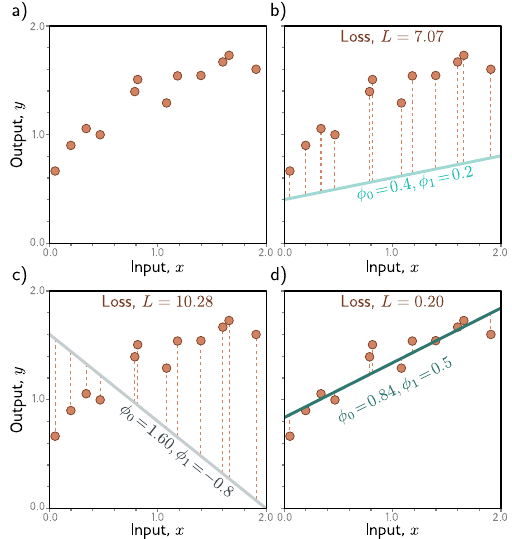
\includegraphics[width=0.7\linewidth]{graficos/desajuste}
		\caption[Ajuste de la función de perdida.]{En (a), los datos de entrenamiento (puntos naranjas) constan de $I = 12$ pares de entrada/salida $[x_i, y_i]$. En (b)-(d), cada panel muestra el modelo de regresión lineal con distintos parámetros. Según la elección de los parámetros de intersección y pendiente $\phi = [\phi_0 , \phi_1]$, los errores del modelo (líneas discontinuas) pueden ser mayores o menores. Los parámetros en las líneas de los paneles (b) y (c) tienen grandes pérdidas $L = 7.07$ y $L = 10.28$, respectivamente, debido a su ajuste pobre. La pérdida $L = 0.20$ en el panel (d) es menor, indicando un mejor ajuste; estos parámetros son los óptimos. Fuente: \protect\parencite{prince2023understanding}.}
		\label{fig:desajuste}
	\end{figure}
	
	
	\begin{figure}[h!]
		\centering
		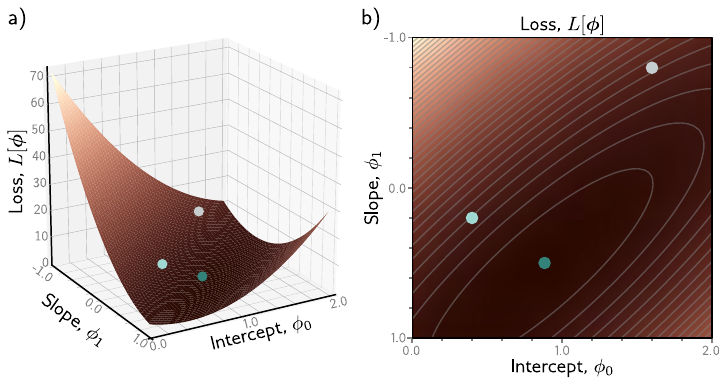
\includegraphics[width=0.7\linewidth]{graficos/loss}
		\caption[Visualización de la función de perdida.]{a) Cada combinación de parámetros $\phi = [\phi_0, \phi_1]$ tiene una pérdida asociada, la función de pérdida resultante $L[\phi]$ puede visualizarse como una superficie. En la figura, los tres círculos representan las tres líneas de la Figura \ref{fig:desajuste}b-d. b) La pérdida también puede visualizarse como un mapa de calor, donde las regiones más brillantes representan pérdidas mayores. El círculo verde tiene los parámetros con la menor pérdida. Fuente: \parencite{prince2023understanding}.}
		\label{fig:loss}
	\end{figure}
	
	
	
	
	%a) Cada convinación de parametros $\phi = [\phi_0 , \phi_1]$ tiene una perdida asociada, la función de perdida resultante $L[\phi]$ puede vizualizarse como una superficie, en la Figura los tres circulos representan las tres lineas de la Figura \ref{fig:desajuste}b-d,  b) La pérdida también se puede vizualizar como un mapa de calor, donde las regiones más brillantes representan perdidas mayores, el circulo verde tiene los párametros con la menor pérdida.
	
	\subsection{Entrenamiento}
	El proceso de encontrar los parámetros que minimicen la pérdida se llama ajuste del modelo o entrenamiento. Inicialmente, los parámetros se seleccionan al azar, y luego se ajustan utilizando la función de pérdida hasta llegar al mínimo, como se ilustra en la figura. Un enfoque común es calcular el gradiente de la superficie en la posición actual y dar un paso en la dirección de mayor descenso, lo que permite optimizar progresivamente los parámetros \parencite{prince2023understanding}. 
	
	\begin{figure}[h!]
		\centering
		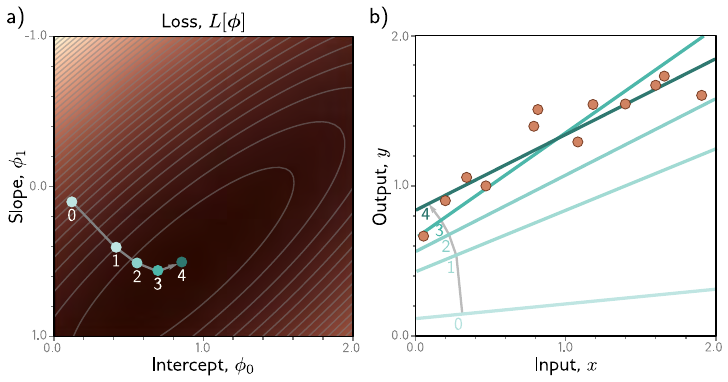
\includegraphics[width=0.7\linewidth]{graficos/loss2}
		\caption[Ajuste de la función de perdida en el entrenamiento.]{a) Algoritmos de entrenamiento iterativos inicializan los parámetros aleatoriamente y luego los mejoran «caminando cuesta abajo» hasta que ya no se puedan mejorar más. Aquí, empezamos en la posición 0 y nos movemos una cierta distancia cuesta abajo (perpendicular a las curvas de nivel) hasta la posición 1. A continuación, volvemos a calcular la dirección cuesta abajo y nos desplazamos a la posición 2. Finalmente alcanzamos el mínimo de la función (posición 4). b) Cada posición 0-4 del panel (a) corresponde a una intersección y una pendiente diferentes y, por lo tanto, representa una línea diferente. A medida que disminuye la pérdida, las líneas se ajustan más a los datos.Fuente: \parencite{prince2023understanding}.}
		\label{fig:loss2}
	\end{figure}
	
	\subsection{Testeo}
	Una vez que el modelo ha sido entrenado, es importante evaluar su rendimiento en el mundo real. Esto se hace calculando la pérdida sobre un conjunto de datos de prueba. La capacidad del modelo para generalizar sus predicciones depende de cuán representativos y completos sean los datos de entrenamiento. Sin embargo, también depende de la complejidad del modelo. Un modelo demasiado simple podría no capturar correctamente la relación entre entrada y salida (underfitting), mientras que uno demasiado complejo podría ajustarse a peculiaridades irrelevantes de los datos (overfitting) \parencite{prince2023understanding}.
	
	\subsection{Redes Neuronales profundas}
	Son un tipo de modelo de aprendizaje automatico, son ecuaciones que pueden representar una familia extremadamente amplia de relaciones entre la entrada y la salida. Estas redes neuronales profundas pueden procesar entradas muy grandes, de longitud variable y contener vrios tipos de estructura internas. Pueden generar números reales únicos (regresión), números múltiples (regresión multivariable) o probabilodaes sobre una o mas clases (clasificación binaria y multiclase) \parencite{prince2023understanding}. 
	
	\subsection{Aprendizaje no Supervizado}
	El aprendizaje no supervizado la construcción de un modelo a partir de datos de entrada sin las correspondientes etiquetas de salida  se denmina aprendizaje no supervisado, la ausenci ade etiquetas de salida significa que no puede haber "supervición". En lugar de aprender una correspondencia entre la entrada y salida, el objetivo es comprender la estructura de los datos \parencite{prince2023understanding}.
	
	\subsection{Redes neuronales artificiales}
	
	Parte de la inteligencia artificial, inspiradas en las redes neuronales biológicas, similares a las que componen el cerebro humano \parencite{olabe1998redes}, además estas redes neuronales artificiales tienen una composición jerárquica, pues dependen de una capa de entrada, capas ocultas, y capas de salida tal como se muestra en la Figura \ref{fig:estructuraann}; sin embargo, para que estas reden neuronales artificiales funciones adecuadamente, es necesario contar una gran cantidad de datos de entrenamiento para ajustar sus pesos y sesgos \parencite{ibm2021redesneuronales}.
	
	
	\begin{figure}[h!]
		\centering
		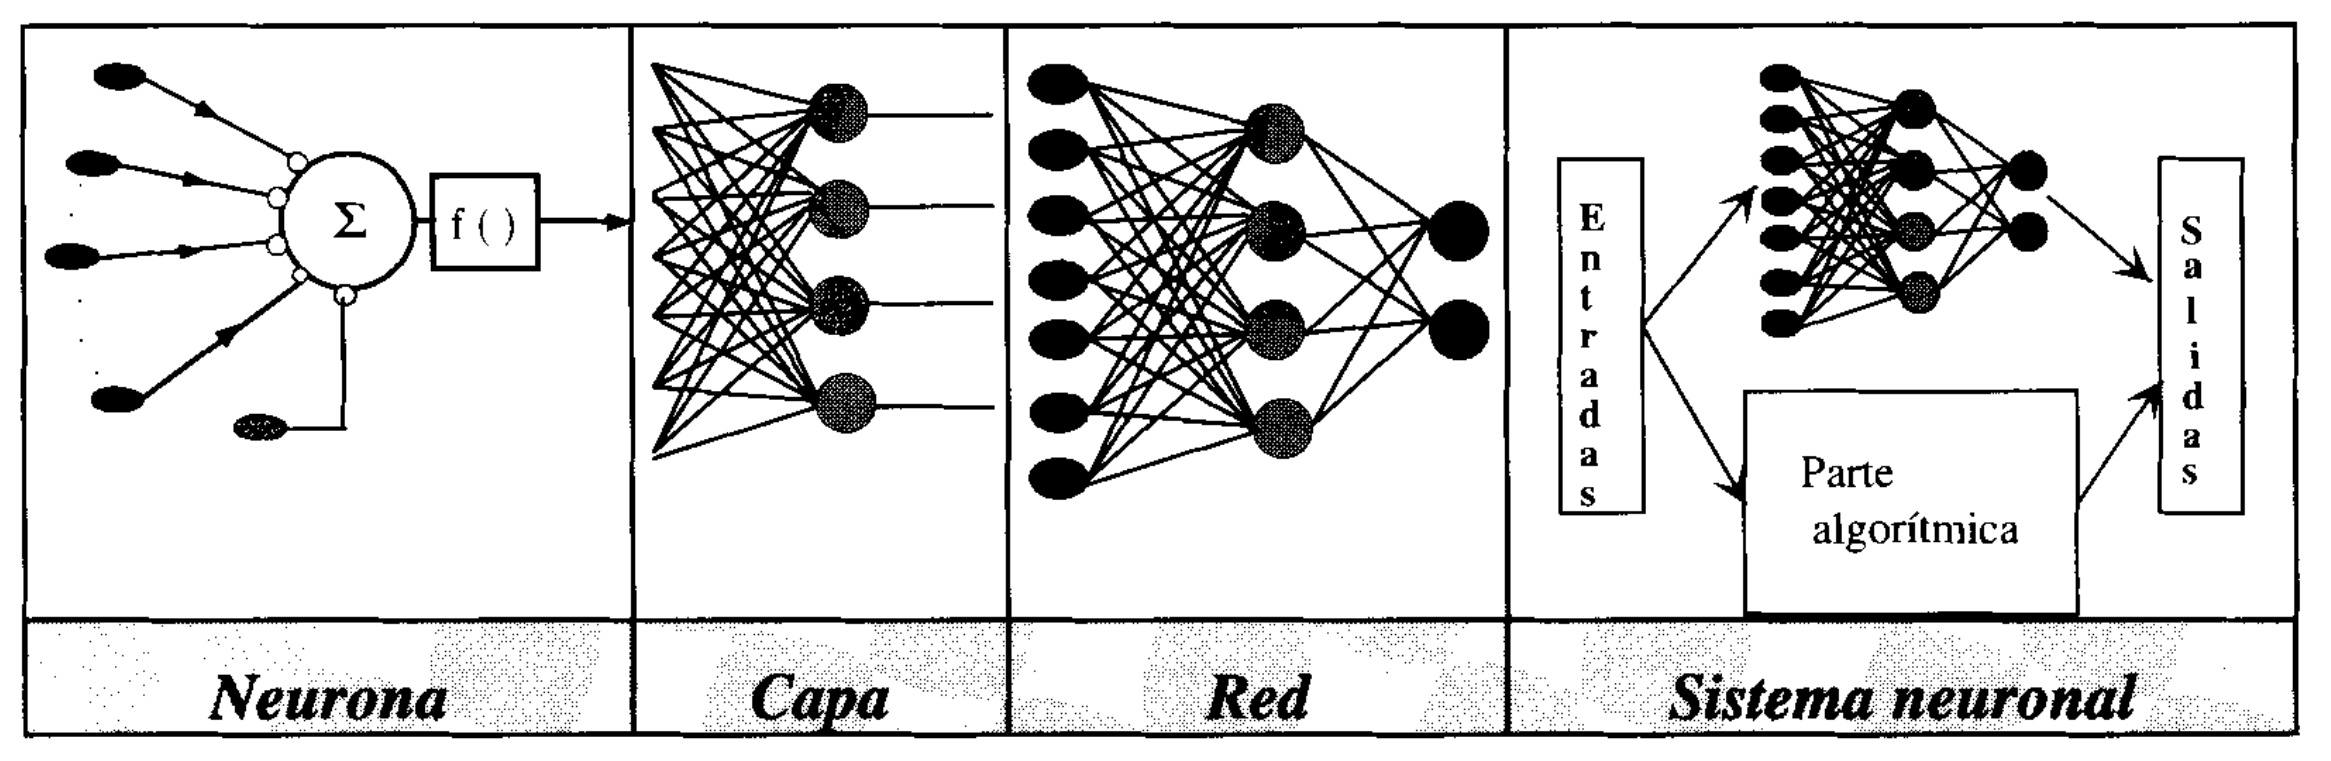
\includegraphics[width=0.7\linewidth]{graficos/estructuraANN}
		\caption[Estructura jerárquica de una ANN]{Estructura jerárquica de una ANN.
			
			Fuente: \parencite{delBrioMolina2001}
		}
		\label{fig:estructuraann}
	\end{figure}
	
	\subsection{Redes Neuronales Convolucionales}	
	
	Es un enfoque de deep learning utilizado para resolver problemas complejos, adecuado para identificar patrones en una imagen (clasificación, segmentación, etc.), supera las imitaciones de enfoques tradicionales de machine learning, además resultan útiles para tratamiento y procesamiento de datos como audio y otros. \parencite{mathworksredneurconvolucional}.
	
	El término "red neuronal convolucional" hace referencia a una red que emplea una operación matemática denominada convolución, que es un tipo especializado de operación lineal. En lugar de la multiplicación de matrices convencional usada en las redes neuronales tradicionales (tipo feedforward), las redes convolucionales utilizan convoluciones en una o más de sus capas \parencite{Goodfellow-et-al-2016}.
	
	Generalmente, la operación utilizada en una red convolucional no se corresponde exactamente con la definición de convolución en campos como la ingeniería o las matemáticas. Normalmente, se denota con un asterisco:
	
	
	\begin{equation}
		\label{eq:cnn1}
		s(t) = (x * w)(t)
	\end{equation}
	
	En terminologia de redes convolucionales, el primer argumento (función x) de la convolución a menudo se denomina entrada, y el segundo argumento (w) como kernel. La salida aveces se denomina mapas de caraceristicas.
	
	El índice de tiempo t puede entonces tomar solo valores enteros. Si ahora suponemis que x y w están definidos solo en el entero t, podemos definir la convolución discreta.
	
	
	\begin{equation}
		\label{eq:cnn2}
		h(t) = (x * w)(t) = \sum_{a=-\infty}^{\infty} x(a) w(t - a)
	\end{equation}
	
	
	En las aplicaciones de machine learning, la entrada suele ser una matriz multidimencional de datos y el kernel suele ser una matriz multidimencional de parámetros que se adaptan mediante el algoritmo de prendizaje. Nos referimos a estas matrices multidimencionales como tensores. Debido a que cada elemento de la entrada y el kernel debe almacernarce explicitamente por separado, generalmente se asumen que estas funciones son cero en todas partes, excepto en el conjunto finito de puntos para los que almacenamos en valores. Esto significa que en la apráctica, podemos implementar la suma infinita como una suma sobre un numero finito de elementos de la matriz \parencite{Goodfellow-et-al-2016}. 
	
	
	\begin{equation}
		\label{eq:cnn3}
		h(i,j) = (X * W)(i,j) = \sum_{m} \sum_{n} X(m,n) W(i-m, j-n)
	\end{equation}
	
	La convolución es conmutativa, lo que significa que podemos escribir de manera equivalente
	
	\begin{equation}
		\label{eq:cnn4}
		h(i, j) = (W * X)(i, j) = \sum_{m} \sum_{n} X(i - m, j - n) W(m, n)
	\end{equation}
	La propiedad conmutativa de la convolución surge porque hemos invertido el kernel en relación con la entrada. La única razón para invertir el kernel es obtener la propiedad conmutativa.
	
	En cambio, muchas bibliotecas de redes neuronales implementan una función relacionada llamada correlación cruzada, que es lo mismo que la convolución pero sin invertir el kernel. Muchas bibliotecas de aprendizaje automático implementan la correlación cruzada pero la llaman convolución. En este texto seguimos esta convención de llamar a ambas operaciones convolución y especificamos si queremos invertir el kernel o no en contextos donde la inversión del kernel es relevante \parencite{Goodfellow-et-al-2016}.
	
	\begin{equation}
		\label{eq:cnn5}
		h(i, j) = (W * X)(i, j) = \sum_{m} \sum_{n} X(i + m, j + n) W(m, n)
	\end{equation}
	
	En el contexto del aprendizaje automático, el algoritmo de aprendizaje aprenderá los valores apropiados del kernel en el lugar apropiado, por lo que un algoritmo basado en convolución con inversión de kernel aprenderá un kernel que esté invertido en relación con el kernel aprendido por un algoritmo sin la inversión \parencite{Goodfellow-et-al-2016}.
	
	Por otro lado, las redes convolucionales, Se usa principalmente para procesar datos de imágenes, las capas convolucionales procesan cada región de imagen local de forma independiente, utilizando párametros compartidos en toda la imagen.
	El kernel convolucional ahora es un objeto 2D. Un kernel cuadrado aplicado a una entrada 2D, que comprende elementos Xij.
	
	Donde W(m,n) son las entradas del kernel convolucional. Esto es simplement una suma ponderada sobre una región de entrada cuadrada, el kernel se traslada tanto horizontal como verticalmente a travéz de la entrada 2D como se observa en la figura \ref{fig:kernel}, para crear una salida en cada posición.
	
	A menudo, la entrada es una imagen RGB, que se trata como una señal en 2D con tres canales tal como se muestra en la figura. Aquí, un kernel de 3x3 tendría pesos 3x3x3 y se aplicaria a los tres canales de entrada en cada una de las 3x3 posiciones para crear una salida 2D que tenga la misma altura y el ancho de la imagen de entrada (suponiendo un padding de cero). Para generar multiples canales de salida, repetimos este proceso con diferentes pesos de kernel y agregamos los resultados par formar un tensor 3D. Si el kernel tiene un tamaño KxK y hay canales de entrada Ci, cada canal de salida es una suma ponderada de catidades CixKxK mas un sesgo (bias). De ello se deduce que para calcular los cnales de calida Co, necesitameos persos CixCoxKxK y sesgos Co \parencite{prince2023understanding}.
	
	 \begin{figure}[h!]
	 	\centering
	 	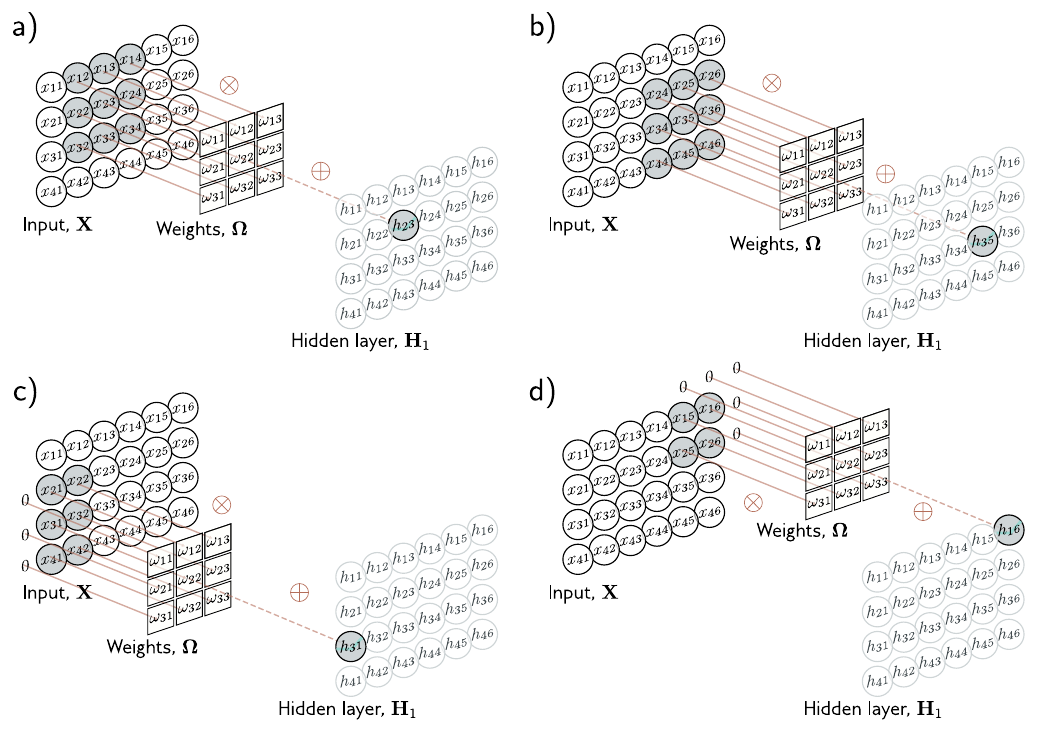
\includegraphics[width=0.7\linewidth]{graficos/kernel}
	 	\caption[Proceso de convolución.]{Cada salida Hij calcula una suma ponderada de 3x3 entradas más cercanas, agrega un sesgo y pasa el resultado a travéz de un a función de activación, a) Aqui, la salida h23 es una suma ponderada de las nueve posiciones desde x12 a x34. b) Se calculan diferentes salidas trasladando el kernel a los largi de la cuadrícula de la imagen en dos dimenciones. c-d) Con padding, las posiciónes más allá del borde de la imagen se concidera cero.
	 		
	 		Fuente: \parencite{prince2023understanding}
	 	}
	 	\label{fig:kernel}
	 \end{figure}
	
	
	\begin{figure}[h!]
		\centering
		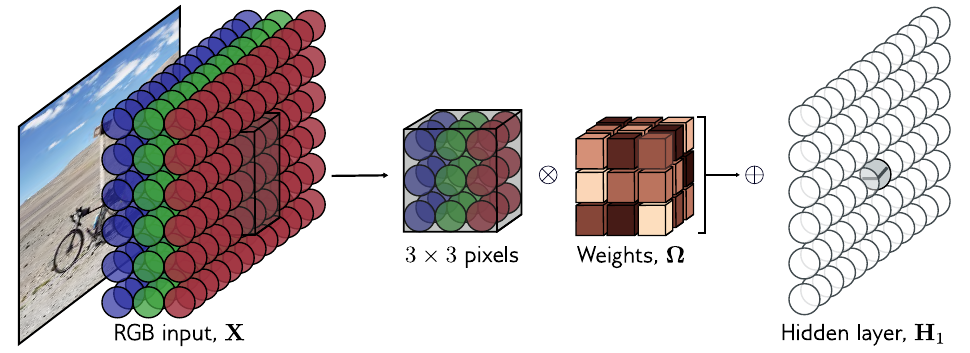
\includegraphics[width=0.7\linewidth]{graficos/kernel2}
		\caption[Convolución 2D aplicado a una imagen RGB]{Convolución 2D aplicado a una imagen, donde la imagen es una entrada de tres canales RGB con un kernel de 3x3, cada preactivación en la capa oculta se calcula multiplicando ppuntualmente los pesos del kernel 3x3x3por el parche de la imagen RGB 3x3 centrado en la misma posición, sumando y añadiendo el sesgo. Para calcular todas las oreactivaciones en la capa oculta, "deslizamos" el kernel sobre la imagen tanto en la dirección horizontal como vertical. La salida es una capa 2D de unidades ocultas. Para crear múltiples canales de salida, se repite este proceso con múltiples kernels, lo que daría como resultado un tensor 3D de unidades ocultas en la capa oculta H1.
			Fuente: \parencite{prince2023understanding}
		}
		\label{fig:kernel2}
	\end{figure}
	 
	
	\begin{figure}[h!]
		\centering
		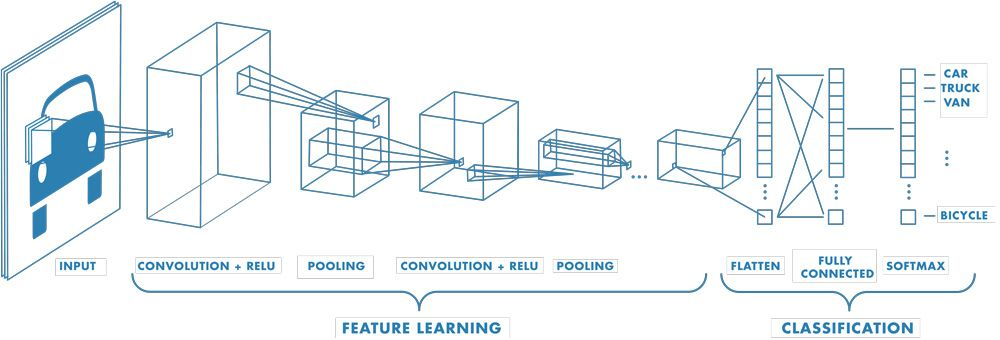
\includegraphics[width=0.7\linewidth]{graficos/CNN}
		\caption[Representación de una CNN]{Representación de una CNN.
		
		Fuente: \parencite{mathworksredneurconvolucional}
		}
		\label{fig:cnn}
	\end{figure}
	
	\subsubsection{Segmentación semántica}
	La segmentación semántica de imágenes es una poderosa técnica de visión por computadora que implica la comprensión y el análisis de las imágenes a nivel de píxeles utilizando algoritmos de aprendisaje profundo. Tiene como objetivo asignar una etiqueta significativa a cada píxel de la imagen, dividiéndola efectivamente en diferentes objetos y/o regiones. A diferencia de la clasificación de imágenes, la cual asigna una sola etiqueta a la imagen completa, la segmentación semántica proporciona una comprensión más detallada y granular del contenido visual dentro de una imagen de acuerdo a diversas categorias. Es clave en aplicaciones como la conducción autónoma y la medicina, donde es necesario identificar áreas relevantes dentro de una imagen. \parencite{herdy_pytorch}.
	\begin{figure}[h!]
		\centering
		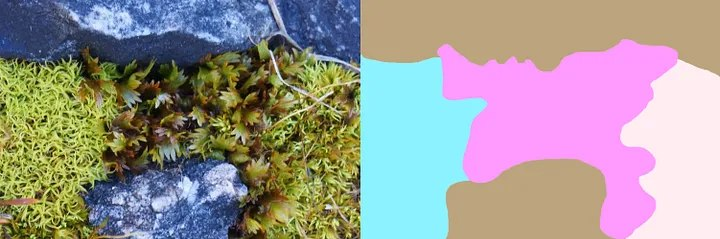
\includegraphics[width=0.7\linewidth]{graficos/segmentation}
		\caption[Segmentación semántica.]{Resultado de la segmentación semántica, el resultado final se crea a partir de los mapas de probabilidad, utilizando un mapa heurístico para encontrar un mapa binario en función de las probabilidades y su proximidad
			espacial. Si hay evidencia suficiente, se agregan las clases subsiguientes y se combinan sus mapas de segmentación.
			
			Fuente: \parencite{herdy_pytorch}
		}
		\label{fig:segmentation}
	\end{figure}
	
	\subsubsection{Arquitecturas de segmentación semántica}
	Existen muchas arquitecturas disponibles que han sido desarrolladas a lo largo de los años, sin embargo, las arquitecturas con un menor número de parámetros son los idóneos para esta investigación.
	
	\subsubsection{U-Net}
	
	U-Net es una arquitectura de red neuronal convolucional diseñada específicamente para segmentación de imágenes biomédicas a nivel de píxel. Desarrollada en 2015 por Olaf Ronneberger, Philipp Fischer y Thomas Brox, U-Net ha tenido un impacto considerable no solo en el ámbito biomédico, sino también en otros campos que requieren segmentación precisa de imágenes. Su estructura simétrica de codificación-decodificación permite la identificación y clasificación de características a diferentes escalas, destacándose por su eficiencia al aprender con conjuntos de datos limitados. Las aplicaciones de U-Net abarcan desde la detección de patrones en teledetección y segmentación de imágenes satelitales hasta la creación de sistemas de apoyo al diagnóstico en medicina, lo que demuestra su versatilidad y capacidad de adaptación \parencite{ronneberger2015u}.
	
	La arquitectura U-Net se distingue por su estructura en forma de U, de donde proviene su nombre. Se compone de un camino de codificación y un camino de decodificación.
	
	\textbf{Camino de codificación}: Esta parte de la red se encarga de capturar el contexto de la imagen de entrada mediante una serie de capas convolucionales y max-pooling, reduciendo la resolución de las dimensiones espaciales y "contrayendo" las imágenes originales.
	
	\textbf{Camino de decodificación}: Esta ruta emplea capas convolucionales y de muestreo ascendente para generar un mapa de segmentación que mantiene las mismas dimensiones espaciales que la imagen de entrada, "expandiendo" las imágenes previamente contraídas.
	

	\begin{figure}[h!]
		\centering
		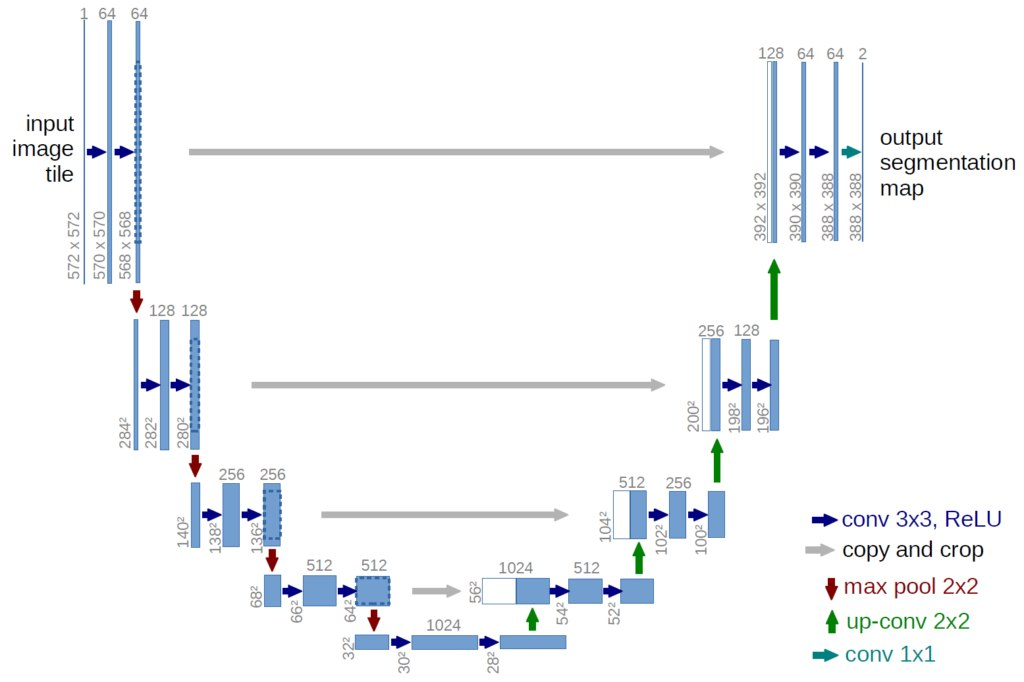
\includegraphics[width=0.7\linewidth]{graficos/unet}
		\caption[Arquitectura U-Net]{Arquitectura U-Net.
			
			Fuente: \parencite{ronneberger2015u}
		}
		\label{fig:unet}
	\end{figure}
	
	La fortaleza de U-Net en la segmentación semántica se debe al uso de conexiones de salto (representadas por las flechas grises en la figura \ref{fig:unet}), que vinculan las rutas de codificación y decodificación al fusionar características. Esto permite conservar los detalles espaciales que se pierden durante la reducción de resolución, manteniendo tanto el contexto local como global de la imagen. Al preservar esta información espacial, U-Net logra máscaras de segmentación más precisas. Estas conexiones de salto permiten que la red capte las relaciones entre las distintas partes de la imagen, mejorando los resultados de segmentación.
	
	La arquitectura U-Net incluye conexiones de salto que facilitan la fusión de características de bajo y alto nivel, lo que mejora la localización. Durante la etapa de reducción de resolución en la arquitectura, antes de realizar el MaxPooling, se guarda el tensor convolucional, que luego se concatena con un tensor muestreado ascendente que tiene la misma dimensión.
	
	\subsubsection{ResUNet}
	
	Inspirados por el aprendizaje profundo residual \parencite{he2016deep} y la arquitectura U-Net \parencite{ronneberger2015u}, \parencite{zhang2018road} propusó el deep residual U-Net, una arquitectura que combina las fortalezas tanto del aprendizaje residual profundo como de U-Net. El deep residual U-Net (ResUnet) se basa en la estructura de U-Net, pero con dos diferencias clave. Primero, en lugar de unidades neuronales simples, utiliza unidades residuales como bloques básicos para construir el deepResUnet. Segundo, se elimina la operación de recorte de la red, lo que resulta en una arquitectura más elegante y con un mejor rendimiento.
	
	Esta combinación trae dos beneficios:
	1) la unidad residual facilitará el entrenamiento de la red; 2) las conexiones salteadas dentro de una unidad residual y entre niveles bajos y altos de la red facilitarán la propagación de información sin degradación, esto permite que el diseño tenga mucho menos parámetros y a su véz lograr rendimientos mucho mejor para la segmentación semántica.

	Sin embargo, entrenar una red neuronal tan profunda es complicado, especialmente cuando los datos de entrenamiento son limitados. Una solución a este problema es utilizar una red preentrenada y luego ajustarla en el conjunto de datos específico. Otra opción es aplicar una amplia data augmentation. Además la estructura de U-Net también ayuda a mitigar las dificultades en el entrenamiento. La idea es que al copiar características de bajo nivel a los niveles superiores correspondientes, se crea un camino que facilita la propagación de información entre los diferentes niveles, lo que no solo mejora la retropropagación durante el entrenamiento, sino que también permite que los detalles finos de bajo nivel complementen las características semánticas de alto nivel. Esta idea guarda cierta similitud con la de las redes neuronales residuales \parencite{he2016deep}. Esto demostró que el rendimiento de U-Net mejoró aún más al reemplazar las unidades simples por unidades residuales.
	
	\textbf{ResidualUnit:} Profundizar en la estructura de una red neuronal multicapa podría mejorar su rendimiento, pero también podría dificultar el entrenamiento, e incluso podría surgir un problema de degradación \parencite{he2016deep}. Para superar estos problemas, \parencite{he2016deep} propusó la red neuronal residual, que facilita el entrenamiento y aborda el problema de degradación. La red neuronal residual está compuesta por una serie de unidades residuales apiladas. Cada unidad residual se puede representar en una forma general.
	
	\begin{equation}
		\label{eq:residual}
		y_l = h(x_l) + F(x_l, W_l)
	\end{equation}
	
	\begin{equation}
		\label{eq:residual2}
		x_{l+1} = f(y_l)
	\end{equation}

	\begin{comment}
	\begin{figure}[h]
		\centering
		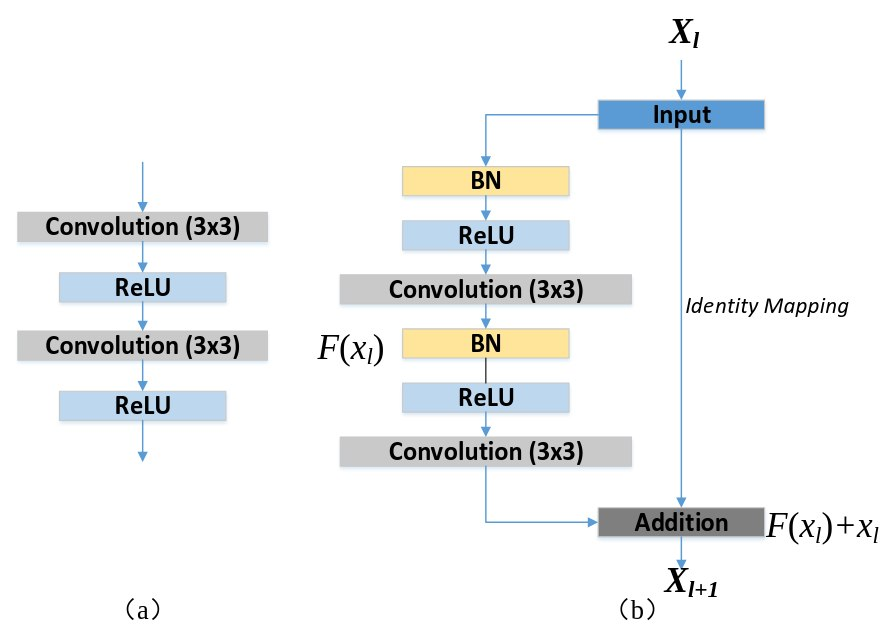
\includegraphics[width=0.7\linewidth]{graficos/residual}
		\caption[Bloques fundamentales de las redes neuronales. (a) Unidad neuronal simple utilizada en U-Net y (b) unidad residual con mapeo de identidad utilizada en el ResUnet propuesto.]{Bloques fundamentales de las redes neuronales. (a) Unidad neuronal simple utilizada en U-Net y (b) unidad residual con mapeo de identidad utilizada en el ResUnet propuesto.
			
			Fuente: \parencite{zhang2018road}
		}
		%\label{fig:residual}
	\end{figure}
	
	\end{comment}

	Donde $x_l$ y $x_{l+1}$ son la entrada y salida de la unidad residual número $l$, $F(.)$ es la función residual, $f(y_l)$ es la función de activación y $h(x_l)$ es una función de mapeo de identidad , donde una opción típica es $h(x_l)=x_l$.La \ref{fig:residual} muestra la diferencia entre una unidad simple y una unidad residual. Dentro de una unidad residual, existen múltiples combinaciones de normalización por lotes (BN), activación ReLU y capas convolucionales. Además se utiliza unidades residuales con preactivación completa para construir el módelo deep residual U-Net.|
	
	\begin{figure}[h!]
		\centering
		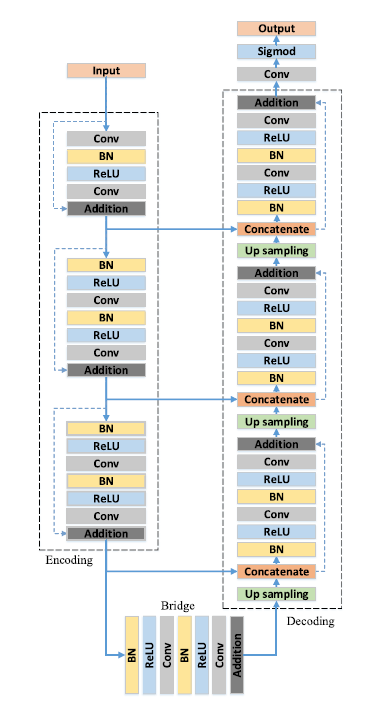
\includegraphics[width=0.5\linewidth]{graficos/ResUNet}
		\caption[Arquitectura profunda ResUnet]{Arquitectura profunda ResUnet.
			
			Fuente: \parencite{ronneberger2015u}
		}
		\label{fig:ResUnet}
	\end{figure}
	
	La arquitectura de DeepResUnet utiliza siete niveles para la extracción de caracteristicas, como se muestra en la figura \ref{fig:ResUnet}, además se compone de tres partes: codificación, puente y decodificación. L aprimera parte codifica la imagen de entrada en representaciones compactas. La última parte recupera las representaciones para una categorización a nivel de píxel, es decir, segmentación semántica. La parte intermedia actúa como un puente que conecta los caminos de codificación y decodificación.Todas las tres partes están construidas con unidades residuales que consisten en dos bloques de convolución de 3 × 3 y un mapeo de identidad.
	
	El camino de codificación y decodificación  tiene tres unidades residuales. Antes de cada unidad, se realiza un muestreo ascendente de los mapas de características del nivel inferior y una concatenación con los mapas de características del camino de codificación correspondiente. Después del último nivel del camino de decodificación, se utiliza una convolución de 1 × 1 y una capa de activación sigmoidea para proyectar los mapas de características multicanal en la segmentación deseada. En total, tenemos 15 capas convolucionales en comparación con las 23 capas de U-Net.


	

	\subsubsection{DeepLabV3}
	
	DeepLabv3+ \parencite{chen2018encoder} es un modelo de redes neuronales completamente convolucionales dilatadas (Dilated FCN) que se utiliza comúnmente para la segmentación semántica, logrando un alto rendimiento en estas tareas. Esta arquitectura mejora el modelo original DeepLabv3 \parencite{chen2017deeplab} al añadir un módulo de decodificación (Decoder). Este módulo Decoder permite integrar mejor las características de bajo y alto nivel, lo que incrementa la precisión en la definición de los bordes de segmentación. La estructura de DeepLabv3+ se representa en la \ref{fig:deeplabv3} y sigue un enfoque global de codificador-decodificador, donde el componente de decodificación es una versión mejorada del DeepLabv3 original, mientras que la parte de codificación es una sección diseñada recientemente. Dentro de la arquitectura del codificador, la estructura principal se basa en Redes Neuronales Convolucionales Profundas (DCNN) que incorporan la convolución dilatada y el componente de Agrupamiento Piramidal Espacial Atrous (ASPP) como elementos clave \parencite{chen2017deeplab}. En esta estructura, la red troncal puede utilizar diferentes arquitecturas, como ResNet, MobileNet y Xception. ResNet, en particular, incluye un bloque de aprendizaje residual que ayuda a abordar el problema de la saturación de precisión y la degradación de rendimiento cuando la profundidad de la red aumenta. Además, investigaciones previas han demostrado que la red ResNet ofrece mejores resultados en segmentación semántica en comparación con otras arquitecturas \parencite{lin2023accurate}.
	
	\begin{figure}[h!]
		\centering
		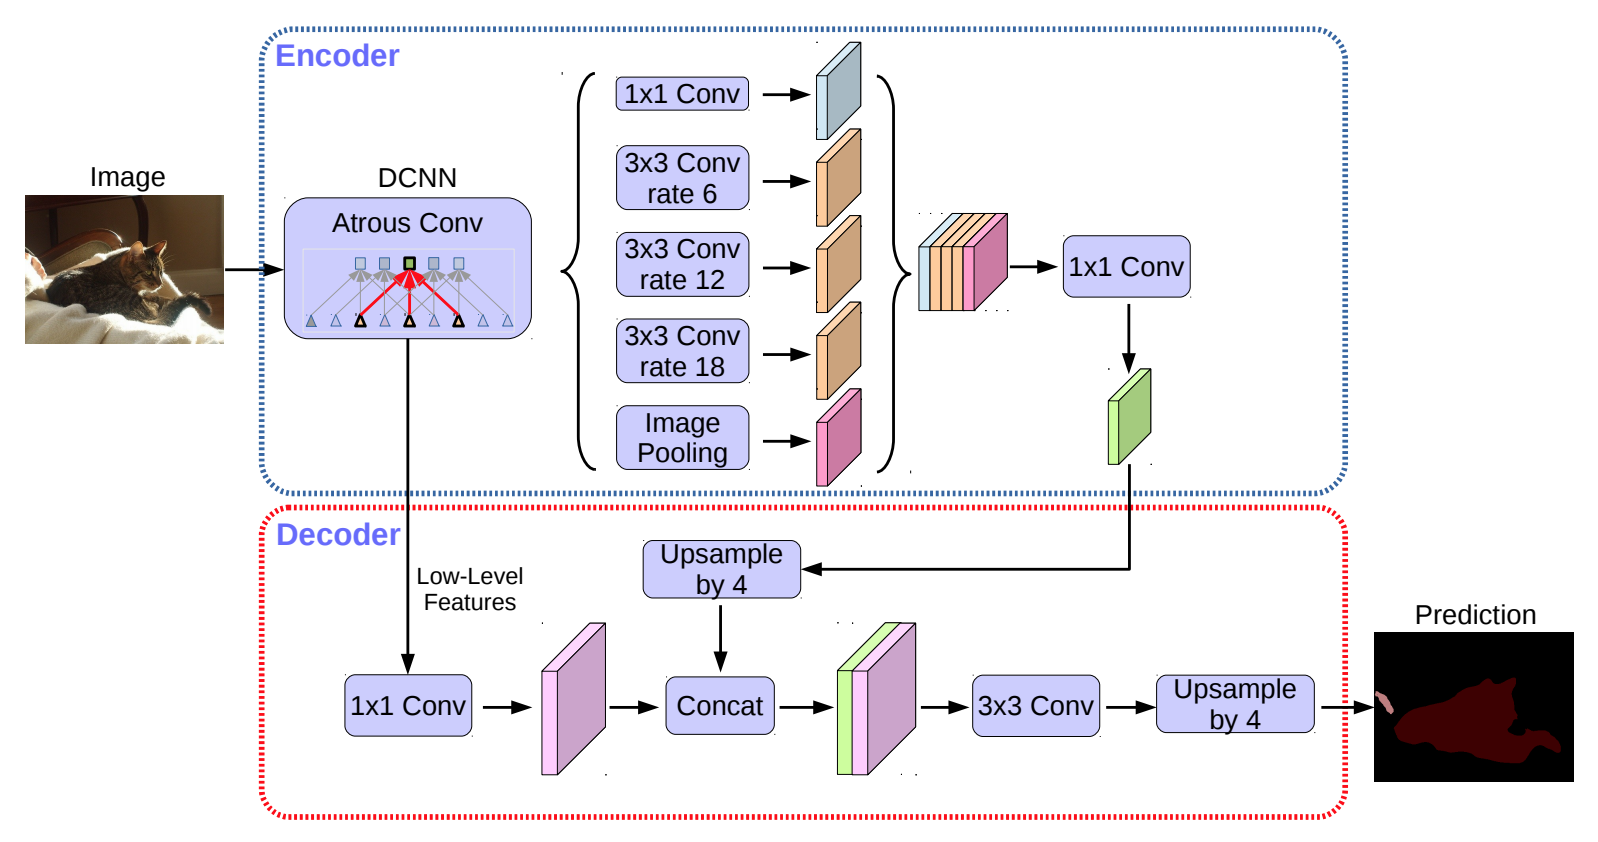
\includegraphics[width=0.7\linewidth]{graficos/deeplabv3}
		\caption[Arquitectura profunda DeepLabV3+]{Arquitectura profunda DeepLabV3+.
			
			Fuente: \parencite{chen2018encoder}
		}
		\label{fig:deeplabv3}
	\end{figure}
	
	
	\textbf{Atrous convolution: }  Es una herramienta poderosa que permite controlar la resolución de las características calculadas por redes neuronales convolucionales profundas y ajustar el campo de visión del filtro para capturar información a múltiples escalas, ejecuta muchas convoluciones con varias tasas de dilatación siguuiendo el codificador, las salidas concatenadas y procesadas de varias convoluciones atrosas se utilizan para crear características ricas en contexto.
	
	Al recopilar datos de diversas escalas y puntos de vista, el módulo ASPP mejora la comprensión de la red de los elementos en una escena. Es especialmente útil para superar los desafíos que presentan los elementos con diferentes tamaños y distribuciones espaciales.
	
\singlespacing
